\documentclass[14pt, a4paper, english]{report}
\usepackage[utf8]{inputenc}
\usepackage[T1]{fontenc,url}
\usepackage{babel,textcomp}
\usepackage{amsmath, amssymb}
\usepackage{polynom}
\usepackage[parfill]{parskip}
\usepackage{titlesec}
\usepackage{fancyhdr}
\usepackage{graphicx}
\usepackage{listings}
\lstset{
	basicstyle=\ttfamily,
	columns=fullflexible,
	frame=single,
	breaklines=true,
	postbreak=\mbox{\textcolor{red}{$\hookrightarrow$}\space},
}
\usepackage{hyperref}
\usepackage{xcolor}
\hypersetup{
	colorlinks   = true, %Colours links instead of ugly boxes
	urlcolor     = blue, %Colour for external hyperlinks
	linkcolor    = blue, %Colour of internal links
	citecolor   = black %Colour of citations
}

% ------------------------------------------------------------
%Bibliografi
\usepackage[style=apa, backend=biber]{biblatex}
\usepackage{csquotes}
\DeclareLanguageMapping{english}{english-apa}
\addbibresource{bibliography.bib}
% ------------------------------------------------------------

% ------------------------------------------------------------
% Side formatering
\lhead{DATA3900}
\chead{Final report}
\rhead{Group 23}
\usepackage{lastpage}
\cfoot{Page \thepage\ of \pageref{LastPage}}
% ------------------------------------------------------------
% ------------------------------------------------------------
\titleformat{\chapter}[display]
  {\normalfont\bfseries}{}{0pt}{\Huge}
%% ------------------------------------------ %% 

% ------------------------------------------------------------
\title
{
	DATA3900 - Bachelorproject \\
	Final report
}
\author{Gruppe 23:\\
    Hansen, Andreas Torres (s338851)\\
	Nguyen, Uy Quoc (s341864)\\
	Ottersland, Anders Hagen (s341883)\\
	\\Total pages: \pageref{LastPage}}
\date{Last updated:\\ \today}

\begin{document}
	\maketitle
	\pagenumbering{gobble}
	\begin{abstract}
		Short summary of the project including the result that the group reached.
	\end{abstract}
	\clearpage
	\chapter*{Preface}
	This is the report of our bachelor thesis at Oslo Metropolitan University, Faculty of Technology, Art and Design. Our project was done for Accenture, and lasted from January 2022 to May 2022. We have tried to develop a solution for traffic management with self-driving cars and server communication. A physical demonstration of our proposed solution is done with the use of a Raspberry Pi computer working as a car. In this project we have documented the functionality of our system, and our process of making it. 
	
	The report is split into 7 chapters. Introduction, research areas, process documentation, implementation, results, discussion and conclusion. At the end we have added a Moscow analysis, sprint overview and our project journal as appendices. Technical terms are in appendix for those with less technical knowledge. (Kan kanskje droppe dette)
	
	We would like to thank everyone that has contributed to our project. We would especially like to thank:
	\begin{itemize}
		\item Ivar Fauske Aasen, Solfrid Johansen and Benjamin Vallestad, representatives from Accenture.
		\item Dr. Jianhua Zhang, internal supervisor at OsloMet.
	\end{itemize}
	\tableofcontents
	% \listoffigures <- utkommenter dersom vi har figurer
	% \listoftables <- utkommenter dersom vi har tabeller
	\clearpage
	\pagestyle{fancy}
	\pagenumbering{arabic}
	% ------------------------------------------------------------
	% Dokumentasjonen går inn her, alt annet generes automatisk. 
	% Husk bare på å inkludere referanser i form av \cite{referanse-navn}
	% uten parantes, eller (\cite{referanse-navn}) <- med parantes
	% ------------------------------------------------------------
	
%	\chapter{Introduction}
\section{Stakeholders}
% \subsection{Contributing members}
\begin{center}
	\begin{tabular}{ll}
		\hline
		&\\
		Name & Role  \\
		&\\
		\hline
		& \\
		Andreas Torres Hansen & Student at OsloMet \\&\\
		Anders Hagen Ottersland & Student at OsloMet\\&\\
		Uy Quoc Nguyen & Student at OsloMet \\&\\&\\
		Benjamin Vallestad & Product owner from Accenture\\&\\&\\
		Ivar Austin Fauske  & Supervisor from Accenture \\&\\
		Solfrid Hagen Johansen & Supervisor from Accenture \\&\\&\\
		Jianhua Zhang & Supervisor from OsloMet\\&\\
		\hline
	\end{tabular}
\end{center}
\subsection{Students}
\begin{itemize}
	\item[] Andreas Torres Hansen, Software Engineering
	\item[] Anders Hagen Ottersland, Software Engineering
	\item[] Uy Quoc Nguyen, Software Engineering
\end{itemize}
\subsection{Product owner}
\begin{itemize}
	\item[] Benjamin Vallestad
\end{itemize}
\subsection{Supervisors}
\begin{itemize}
	\item[] Professor Jianhua Zhang, Internal Supervisor
	\item[] Ivar Austin Fauske, External Supervisor
	\item[] Solfrid Hagen Johansen, External Supervisor
\end{itemize}
\subsection{Client}
\subsubsection*{Accenture AS}

Accenture is an international IT consulting firm that operates in 200 different countries worldwide. The main office is located in Dublin, and the Norwegian main office is in Fornebu. Accenture has 674 thousand employees internationally, of which 1000 work in Norway \parencite{accenture_earning_report_2021}. In 2021, Accenture generated a revenue of approximately \$50.3 billion \parencite{accenture_about}.

\section{Project Description}
\subsection{Project background}
For many years, Accenture has offered innovative bachelor thesis projects for students at OsloMet and Høyskolen Kristiania. In 2020, a group of students from Høyskolen Kristiania was developing model-sized self-driving vehicles using Raspberry Pi in conjunction with machine learning as their project. This year our group was offered to extend this project further; to explore plausible improvement with the addition of a centralized communication system.

According to our product owner, Norway is one of the countries that are ready to utilize self-driving cars. However, self-driving vehicles alone are likely not enough to solve all of today's traffic challenges. Hence, this project aims to solve the issue by introducing a management system for autonomous vehicles and evaluating the value such a system can provide.
\subsection{Significance}
Our project provides value for Accenture in the shape of building knowledge around new technology and theory. Accenture also wants to explore the potential positive societal and climate effects a centralized communication system for transportation could provide.


\subsection{Goals and requirements}
The goal of the project is to end up with a prototype that can be shown to interesents and demonstrate how self-driving cars could be combined with a centralized system. For this we will use the self-driving car that Accenture already owns, as a result of the previous bachelor's-thesis done with them. The conditions are that the product must be possible to present, either as a physical or digital showcase. Preferably, the prototype can show at least one situation where the outcome differs depending on the use of self-driving cars plus a centralized system, versus only using self-driving cars. The system should also be scalable, so that more vehicles can be added or removed at a later point in time. 
\subsection{Problem statement}
Based on the goals and requirements set by Accenture, we have formulated the research and development question:
\begin{quote}
	``How can we improve traffic flow, by using a combination of self-driving cars and a centralized communication system?''
\end{quote}
%	\chapter{Research areas}
\section{Internet of Things (IoT)}
The Internet Of Things refers to physical objects that communicate with the use of sensors, cameras, software or other technologies that connect and exchange data. This communication takes place over the Internet or other communication forms. The number of connected IoT-devices in the world is increasing, and it is becoming a big part of society \parencite{iot_analytics}. The field of IoT has also been evolving in recent years due to other technologies becoming more accessible, such as machine learning.

You need not look further than to the smart-home consumer market to find applications in your life, of devices communicating to solve problems. It could also be applied in climate surveillance systems, energy or transportation. The benefits that an internet of connected devices could add billions in value to industries across the world, and to the global economy. In this thesis we will explore the possibilities of using IoT in transportation, more specifically in personal automobiles. The convergence of these fields is more commonly known as IoV, Internet of Vehicles, and it is a central theme of our thesis. An IoV system is a distributed system for wireless communication and information exchange between vehicles through agreed upon communication protocols \parencite{chinese_iov}.  The system could potentially integrate functionality for dynamic information exchange, vehicle control and  smart traffic management. In our thesis we will explore these possibilities on a small scale, with the hopes of making a solution that can be scaled up at a later point. 

Challenges to be aware of with IoT-systems, and consequently also IoV-systems include, among others, ethical questions about decision-making, physical and digital safety for humans and infrastructure, storage of data and power usage. With the evolution, and increased availability of artificial intelligence (AI), IoT has also evolved to implement algorithms powered by AI. We will discuss the implementation of AI and machine learning further down in the thesis, but it is possible to view some of the problems with IoV-systems as an extension of typical problems with AI systems. In our work with the thesis we have kept these challenges in mind when formulating proposed solutions, and it has affected how we have worked.

\section{Artificial Intelligence (AI)}
Artificial intelligence(AI) leverages computers and machines to mimic the problem-solving and decision-making capabilities of the human mind. At its simplest form, artificial intelligence is a field, which combines computer science and robust datasets, to enable problem-solving \parencite{artificial_intelligence}. There are two types of Ai, weak Ai and strong Ai. Weak AI, also known as narrow AI, is trained to perform specific tasks such as, voice recognition, data labeling, and in our case, driving cars. Narrow AI is the most common type of AI, and the type used in today's AI systems. 

Strong AI is made up of Artificial General Intelligence (AGI) and Artificial Super Intelligence (ASI) \parencite{artificial_intelligence}. General AI is a theoretical form of AI where a machine would have reached the same level of intelligence as a human being. Artificial Super intelligence is a theoretical form of AI where the machine has surpassed the intelligence of humans. This type of AI is often presented in movies. 
\section{Machine learning}
Machine learning is a subfield of artificial intelligence, which is broadly defined as the capability of a machine to imitate intelligent human behavior \parencite{ml_explained}.

There are three types of machine learning, supervised learning, unsupervised learning and reinforcement learning. In supervised machine learning the algorithm is given labeled data to help predict outcomes. This means the algorithm uses already historical data. Supervised learning is the most commonly used machine learning. Supervised learning can be separated into 2 different problems when data mining, classification and regression \parencite{delua_ibm}. Classification uses an algorithm that assigns test data into the right categories. For example, differentiate between cats and dogs. Regression is another type of supervised learning method that uses an algorithm to understand the relationship between dependent and independent variables \parencite{delua_ibm}. Regression is used for predicting mathematical values such as stocks and sales. The prior group used supervised learning to train their camera detection model. 

However in unsupervised learning the algorithm uses non-labeled data. The algorithm looks for patterns or trends in the data. This can be used for labeling data or figuring out trends. Customers that buy item x will be more likely to buy item y as well.

Reinforcement learning trains the machine via trial and error and a reward system. This is commonly used to train machines in games or autonomous vehicles. An example is Stockfish 14, one of the best chess engines in the world. (kilde)


About four of five traffic accidents are caused by human error \parencite{policy_advise}. And in fields that require a specific task to be done, for example chess ai, already surpasses humans. This means if an learns to drive perfectly, four out of five traffic accidents can be avoided. However driving is a complex task that requires a ton of data, and decision making. In addition, for an Ai to give the most accurate outcome a lot of accurate test data are required. Nearly 43\% of people in the US are afraid of self-driving cars \parencite{kopestinsky}. Giving a self-driving car an accurate driving environment without risking human lives is therefore a challenge.
\section{Self driving cars}
Autonomous vehicles also known as self-driving cars are becoming more and more relevant. We see huge companies such as Tesla and Ruter investing into research. Ruter has implemented a short route that is part of Ruter’s transport system where there are only self driving buses. Even though it’s unclear exactly when fully automated vehicles will hit the roads it seems like the day is getting closer and closer. It’s impossible to predict exactly what's going to occur in a traffic scenario. That’s why the use of AI is prefered compared to traditional computing in this setting. 

The Society of Automotive Engineers (SAE) currently defines 6 levels of driving automation ranging from Level 0 (fully manual) to Level 5 (fully autonomous) \parencite{synopsys_autonomous_car}. The self driving buses Ruter has implemented is at the third level of automation. This means that there is a driver present to take over if something goes wrong. In this project we will mainly focus on the 4th level of automation. In the fourth level of automatization there is no driver present and the car is fully automated in a specific setting, in our case, a prebuilt track. What differentiate the fourth and the fifth level is that in the fifth level the vehicles can drive in any setting.
\section{Ethics and security}
For an Ai to be able to train there will be a need for training data. Therefore a database saving information about the trips will be needed, in the IoT-system, for the AI to further improve.

When there is saving of data involved it is important to consider personal information. Personal information typically includes name, address, phone number, email and date of birth \parencite{datatilsynet_personopplysning}. In addition it also includes behavioral patterns, for example where you drive to work each day or where you go shopping. In this case, an IoT system that saves the car's trips it’s considered saving of personal information. The system could try to anonymize the data, but there will still be possibilities to find patterns in the data. You are allowed to save some personal information as long as you follow certain rules. 

Hackers are a problem when it comes to systems controlling entities that can affect human lives. If hackers were able to get control of such a system it could lead to a lot of damage. It is therefore important for a secure security system to be in place. If anyone were to breach the system, it would have to detect that it has been breached, and shut down so the cars can move on their own without the system.


%	\chapter{Work methodology and technology used}
\section{Development method}
We had very few requirements and technical restrictions when we received the project, which left the project open to interpretation. Therefore, we wanted to choose a flexible work methodology. Agile work methods focus on continuous planning throughout the process and having frequent communication with the client, in our case Accenture. We had meetings with our external supervisors from Accenture once every second week, which meant the agile model was a good fit for our project. We took inspiration from two light frameworks, Scrum and Kanban.

We took inspiration from two light frameworks, Kanban and Scrum. Scrum is an agile,  light framework that helps people and teams work together. Scrum describes a set of meetings, roles, and tools. 

A sprint is an essential part of using the Scrum framework. Sprints are a fixed time length, often between one and four weeks. In this specified time length, the teams do tasks assigned from the sprint backlog. Each sprint starts with sprint planning and ends with a sprint retrospective. We found it most viable for our project to plan in increments of two weeks. We chose two-week increments because we felt it was an even balance between work and planning. As mentioned, we also had meetings with our client Accenture every two weeks, which fitted well with the time increment.   

\subsection{Scrum and sprints}\label{section:scrum}
Scrum is a framework that dictates how developers work in teams to solve complex problems. The development process is also divided into time intervals called a sprint. A sprint is an essential part of using the Scrum framework \parencite{prosjektveilederen}. Sprints are a fixed time length, often between one and four weeks. In this specified time length, the teams do tasks assigned from the sprint backlog. Each sprint starts with sprint planning and ends with a sprint retrospective.

We found it most viable for our project to plan in increments of two weeks. We chose two-week increments because we felt it was an even balance between work and planning. This time increment also fitted our bi-weekly meeting plan with our supervisors.

Our group also used the meetings in the Scrum framework, which consist of sprint planning, sprint retrospective, and daily standups. Sprint planning is a meeting or event which starts before a sprint. During sprint planning, teams agree on goals for the sprint and what tasks from the backlog should be prioritized. The backlog is a list of functionality the product should contain. In addition, we wrote down the tasks for the specific sprints in Google Docs. These tasks were to be finished by the next sprint. \figref{fig:sprintoverview} shows our sprint planning document that lists our goals for each sprint.

\begin{figure}[h!]
	\centering
	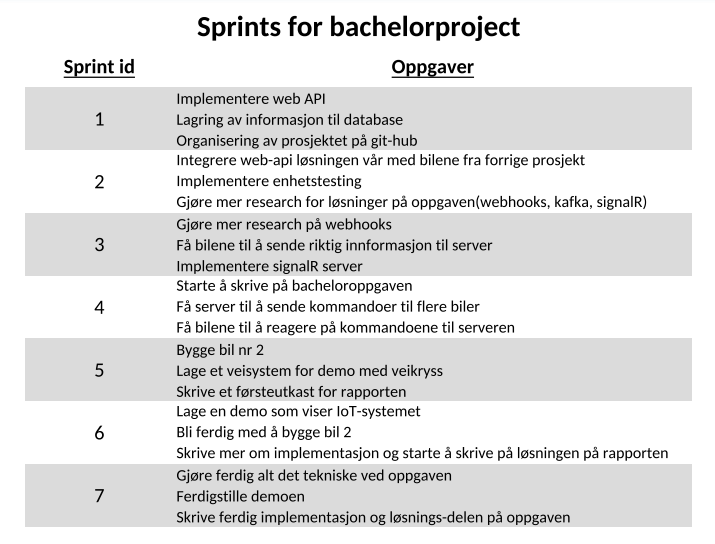
\includegraphics[width=1\linewidth]{figures/Sprint_overview}
	\caption[Sprint overview]{An overview of our sprints. Each sprint lasted 2 weeks. This figure shows the main tasks of each sprint.}
	\label{fig:sprintoverview}
\end{figure}

After a sprint, we would have a sprint retrospective to discuss what went well and what we could have done better. We would also examine if the task assigned in the sprint meetings was finished or needed more work. These meetings helped us reflect over the prior week and adjust accordingly, if necessary. The sessions also helped us determine if we were on track with our initial plan. 
 
In addition to the weekly meetings, we also had daily standups. Daily standups are short meetings, usually lasting around five minutes, where each person answers three questions:
\begin{itemize}
	\item What did the person do last time? 
	\item What is the person going to do today? 
	\item Are there any challenges?
\end{itemize}
We implemented daily standups because it helped our team get on the same page, and it made it easier to plan what each of us had to do that specific day.

Scrum often consists of a team with different roles. As a team of three, we did not feel the necessity to have specified roles because we usually worked together on our projects. However, we alternated on being the scrum master. The scrum master's responsibility is to keep track of the backlog and lead the sprint planning meetings.

\subsection{Kanban as our backlog}
Our implementation of Kanban was to use a Kanban board as the backlog. We used a Kanban board to visualize where a task is in the work process. \figref{fig:kanbanscreenshot} shows an example from our project, with description labels and priority labels:
\begin{figure}[h!]
	\centering
	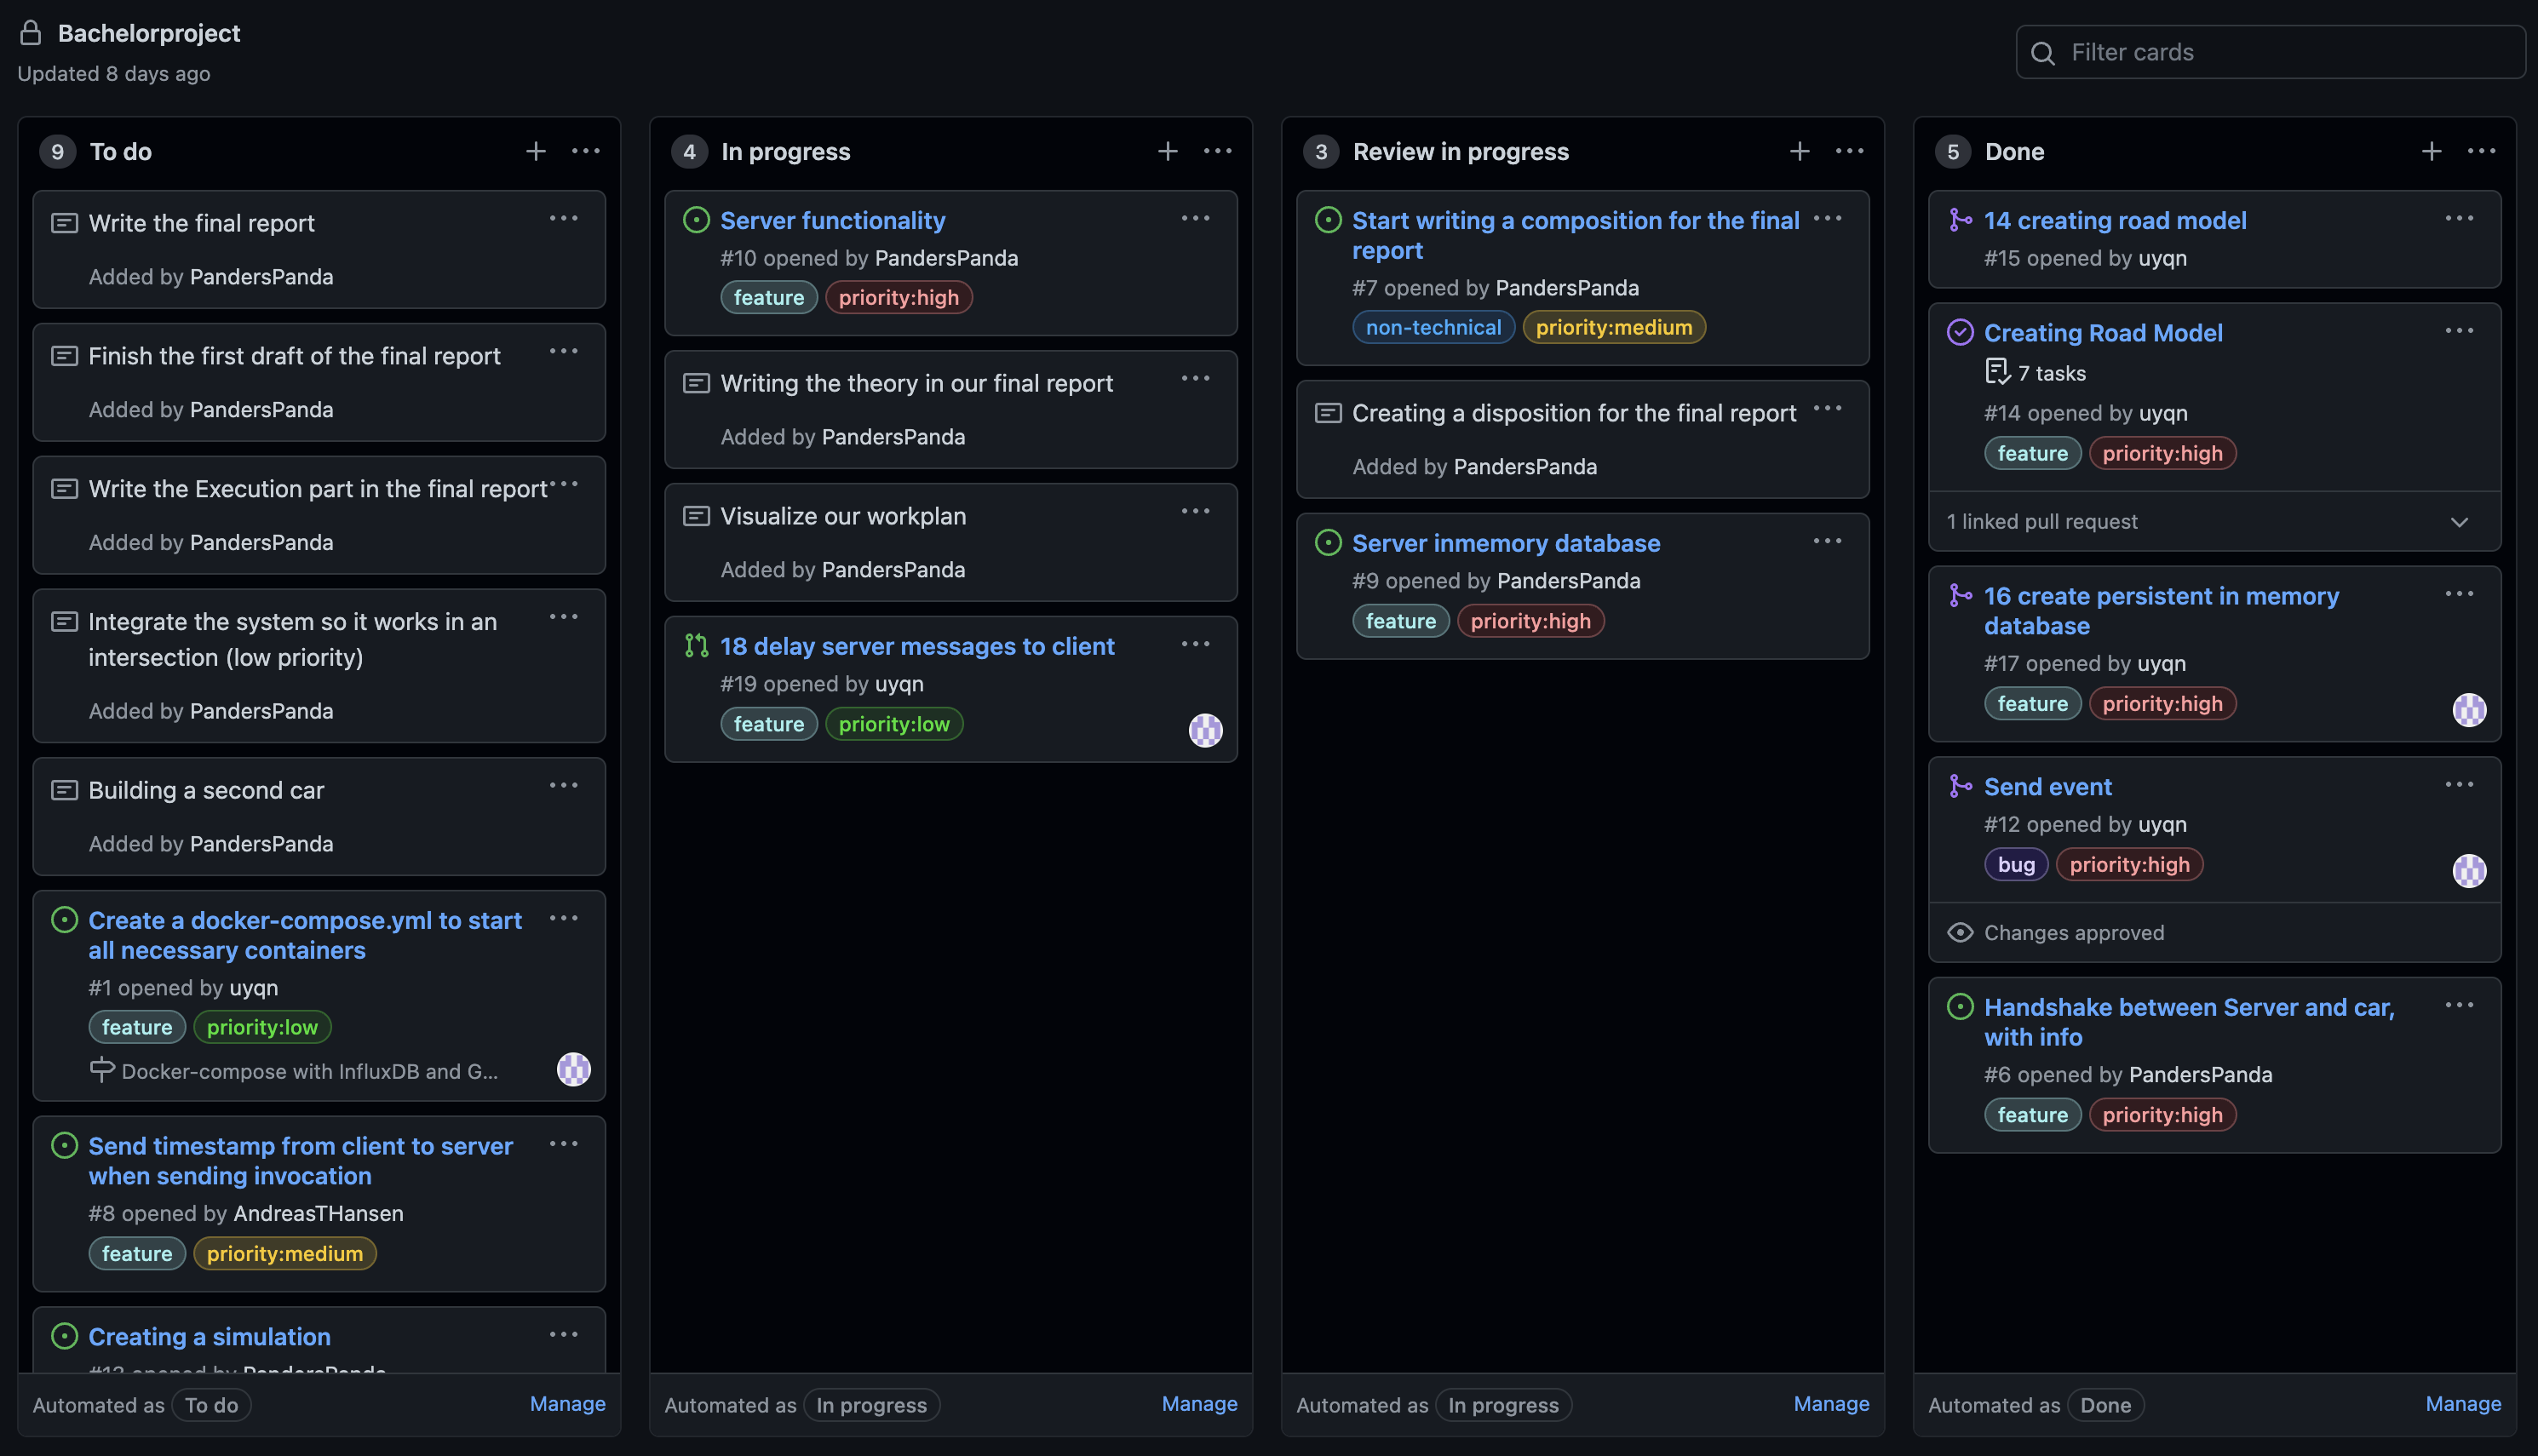
\includegraphics[width=1\linewidth]{figures/kanban_screenshot}
	\caption[kanban screenshot]{Extract of our Kanban board from Github. Each task has a color-coded label representing the priority, and a label to describe the task.}
	\label{fig:kanbanscreenshot}
\end{figure}

We have four columns that represent which phase a task is in. The backlog is the tasks in the to-do column. We dragged it over to the "In progress"-column when we were working on a task. After finishing a task, it went to the "Review in progress"-column, where we reviewed it. If we concluded that the task was finished in the reviewing, it was dragged over to the "Done"-column. Whenever a task is created we tagged it with a high, medium or low to indicate its priority. In addition, to the priority tag, we also gave each task a label; feature, bug, and non-technical to communicate what the task entails. You can also connect the tasks to a specific branch, so the task automatically gets finished when merging the branch into the main branch. The Kanban board was a great tool to see which tasks to choose for our sprints and also keep track of where the tasks were in their process.

However, we did not use the Kanban board throughout the whole process. This is because the backlog was changing a lot, and the Kanban board needed many modifications to be up to date. We figured out that it was more beneficial to focus on one framework, which in our case was Scrum. In addition, we were able to keep track of the tasks by having frequent meetings. 
\section{Tools and technologies}
The circumstances surrounding Covid 19 meant that we could not meet our supervisors in person at the start. Luckily, the group could still meet physically a few times a week. We had to use a wide range of tools for communication. Most restrictions were removed later in the project, but we kept our meetings with our supervisors digital throughout the project. 

\begin{itemize}
	\item Email - Formal communication with supervisors and product owner
	\item Teams - Meetings, and the platform of choice for communicating with the external supervisors on an informal level. 
	\item Zoom - Meetings with our internal supervisor at OsloMet
	\item Facebook Messenger - Communication internally in the group. We used it to send messages to each other when we were not physically together, and to send pictures of code. 
\end{itemize}

The project required us to collaborate while working on different computers, leading to potential overlapping. Therefore, tools that helped us work on the project together were essential. We used the following tools for this purpose:

\begin{itemize}
	\item Git and Github - Version control of choice
	\item Google docs - Used to write our journal and other documents that need to get updated regularly, and to share documents. 
	\item Latex - Used to write reports.
\end{itemize}

We also needed text editors that supported the programming languages that we used. Our solution was created with Python and C\#.
\begin{itemize}
	\item Pycharm - IDE for coding in Python
	\item Visual studio and Rider - IDE for coding in C\#
	\item Thonny - Text editor for coding in Python on Raspberry pi
\end{itemize}

Project planning and documentation were also an important part of the project. The tools we used for the project planning were:

\begin{itemize}
	\item Github project - Kanban board and creating backlog tasks
	\item Excel - Used for visualizing our workplan with tables and a Gantt diagram
\end{itemize}
%	\chapter{Introduction}
\section{Stakeholders}
% \subsection{Contributing members}
\begin{center}
	\begin{tabular}{ll}
		\hline
		&\\
		Name & Role  \\
		&\\
		\hline
		& \\
		Andreas Torres Hansen & Student at OsloMet \\&\\
		Anders Hagen Ottersland & Student at OsloMet\\&\\
		Uy Quoc Nguyen & Student at OsloMet \\&\\&\\
		Benjamin Vallestad & Product owner from Accenture\\&\\&\\
		Ivar Austin Fauske  & Supervisor from Accenture \\&\\
		Solfrid Hagen Johansen & Supervisor from Accenture \\&\\&\\
		Jianhua Zhang & Supervisor from OsloMet\\&\\
		\hline
	\end{tabular}
\end{center}
\subsection{Students}
\begin{itemize}
	\item[] Andreas Torres Hansen, Software Engineering
	\item[] Anders Hagen Ottersland, Software Engineering
	\item[] Uy Quoc Nguyen, Software Engineering
\end{itemize}
\subsection{Product owner}
\begin{itemize}
	\item[] Benjamin Vallestad
\end{itemize}
\subsection{Supervisors}
\begin{itemize}
	\item[] Professor Jianhua Zhang, Internal Supervisor
	\item[] Ivar Austin Fauske, External Supervisor
	\item[] Solfrid Hagen Johansen, External Supervisor
\end{itemize}
\subsection{Client}
\subsubsection*{Accenture AS}

Accenture is an international IT consulting firm that operates in 200 different countries worldwide. The main office is located in Dublin, and the Norwegian main office is in Fornebu. Accenture has 674 thousand employees internationally, of which 1000 work in Norway \parencite{accenture_earning_report_2021}. In 2021, Accenture generated a revenue of approximately \$50.3 billion \parencite{accenture_about}.

\section{Project Description}
\subsection{Project background}
For many years, Accenture has offered innovative bachelor thesis projects for students at OsloMet and Høyskolen Kristiania. In 2020, a group of students from Høyskolen Kristiania was developing model-sized self-driving vehicles using Raspberry Pi in conjunction with machine learning as their project. This year our group was offered to extend this project further; to explore plausible improvement with the addition of a centralized communication system.

According to our product owner, Norway is one of the countries that are ready to utilize self-driving cars. However, self-driving vehicles alone are likely not enough to solve all of today's traffic challenges. Hence, this project aims to solve the issue by introducing a management system for autonomous vehicles and evaluating the value such a system can provide.
\subsection{Significance}
Our project provides value for Accenture in the shape of building knowledge around new technology and theory. Accenture also wants to explore the potential positive societal and climate effects a centralized communication system for transportation could provide.


\subsection{Goals and requirements}
The goal of the project is to end up with a prototype that can be shown to interesents and demonstrate how self-driving cars could be combined with a centralized system. For this we will use the self-driving car that Accenture already owns, as a result of the previous bachelor's-thesis done with them. The conditions are that the product must be possible to present, either as a physical or digital showcase. Preferably, the prototype can show at least one situation where the outcome differs depending on the use of self-driving cars plus a centralized system, versus only using self-driving cars. The system should also be scalable, so that more vehicles can be added or removed at a later point in time. 
\subsection{Problem statement}
Based on the goals and requirements set by Accenture, we have formulated the research and development question:
\begin{quote}
	``How can we improve traffic flow, by using a combination of self-driving cars and a centralized communication system?''
\end{quote}
	%\chapter{Research areas}
\section{Internet of Things (IoT)}
The Internet Of Things refers to physical objects that communicate with the use of sensors, cameras, software or other technologies that connect and exchange data. This communication takes place over the Internet or other communication forms. The number of connected IoT-devices in the world is increasing, and it is becoming a big part of society \parencite{iot_analytics}. The field of IoT has also been evolving in recent years due to other technologies becoming more accessible, such as machine learning.

You need not look further than to the smart-home consumer market to find applications in your life, of devices communicating to solve problems. It could also be applied in climate surveillance systems, energy or transportation. The benefits that an internet of connected devices could add billions in value to industries across the world, and to the global economy. In this thesis we will explore the possibilities of using IoT in transportation, more specifically in personal automobiles. The convergence of these fields is more commonly known as IoV, Internet of Vehicles, and it is a central theme of our thesis. An IoV system is a distributed system for wireless communication and information exchange between vehicles through agreed upon communication protocols \parencite{chinese_iov}.  The system could potentially integrate functionality for dynamic information exchange, vehicle control and  smart traffic management. In our thesis we will explore these possibilities on a small scale, with the hopes of making a solution that can be scaled up at a later point. 

Challenges to be aware of with IoT-systems, and consequently also IoV-systems include, among others, ethical questions about decision-making, physical and digital safety for humans and infrastructure, storage of data and power usage. With the evolution, and increased availability of artificial intelligence (AI), IoT has also evolved to implement algorithms powered by AI. We will discuss the implementation of AI and machine learning further down in the thesis, but it is possible to view some of the problems with IoV-systems as an extension of typical problems with AI systems. In our work with the thesis we have kept these challenges in mind when formulating proposed solutions, and it has affected how we have worked.

\section{Artificial Intelligence (AI)}
Artificial intelligence(AI) leverages computers and machines to mimic the problem-solving and decision-making capabilities of the human mind. At its simplest form, artificial intelligence is a field, which combines computer science and robust datasets, to enable problem-solving \parencite{artificial_intelligence}. There are two types of Ai, weak Ai and strong Ai. Weak AI, also known as narrow AI, is trained to perform specific tasks such as, voice recognition, data labeling, and in our case, driving cars. Narrow AI is the most common type of AI, and the type used in today's AI systems. 

Strong AI is made up of Artificial General Intelligence (AGI) and Artificial Super Intelligence (ASI) \parencite{artificial_intelligence}. General AI is a theoretical form of AI where a machine would have reached the same level of intelligence as a human being. Artificial Super intelligence is a theoretical form of AI where the machine has surpassed the intelligence of humans. This type of AI is often presented in movies. 
\section{Machine learning}
Machine learning is a subfield of artificial intelligence, which is broadly defined as the capability of a machine to imitate intelligent human behavior \parencite{ml_explained}.

There are three types of machine learning, supervised learning, unsupervised learning and reinforcement learning. In supervised machine learning the algorithm is given labeled data to help predict outcomes. This means the algorithm uses already historical data. Supervised learning is the most commonly used machine learning. Supervised learning can be separated into 2 different problems when data mining, classification and regression \parencite{delua_ibm}. Classification uses an algorithm that assigns test data into the right categories. For example, differentiate between cats and dogs. Regression is another type of supervised learning method that uses an algorithm to understand the relationship between dependent and independent variables \parencite{delua_ibm}. Regression is used for predicting mathematical values such as stocks and sales. The prior group used supervised learning to train their camera detection model. 

However in unsupervised learning the algorithm uses non-labeled data. The algorithm looks for patterns or trends in the data. This can be used for labeling data or figuring out trends. Customers that buy item x will be more likely to buy item y as well.

Reinforcement learning trains the machine via trial and error and a reward system. This is commonly used to train machines in games or autonomous vehicles. An example is Stockfish 14, one of the best chess engines in the world. (kilde)


About four of five traffic accidents are caused by human error \parencite{policy_advise}. And in fields that require a specific task to be done, for example chess ai, already surpasses humans. This means if an learns to drive perfectly, four out of five traffic accidents can be avoided. However driving is a complex task that requires a ton of data, and decision making. In addition, for an Ai to give the most accurate outcome a lot of accurate test data are required. Nearly 43\% of people in the US are afraid of self-driving cars \parencite{kopestinsky}. Giving a self-driving car an accurate driving environment without risking human lives is therefore a challenge.
\section{Self driving cars}
Autonomous vehicles also known as self-driving cars are becoming more and more relevant. We see huge companies such as Tesla and Ruter investing into research. Ruter has implemented a short route that is part of Ruter’s transport system where there are only self driving buses. Even though it’s unclear exactly when fully automated vehicles will hit the roads it seems like the day is getting closer and closer. It’s impossible to predict exactly what's going to occur in a traffic scenario. That’s why the use of AI is prefered compared to traditional computing in this setting. 

The Society of Automotive Engineers (SAE) currently defines 6 levels of driving automation ranging from Level 0 (fully manual) to Level 5 (fully autonomous) \parencite{synopsys_autonomous_car}. The self driving buses Ruter has implemented is at the third level of automation. This means that there is a driver present to take over if something goes wrong. In this project we will mainly focus on the 4th level of automation. In the fourth level of automatization there is no driver present and the car is fully automated in a specific setting, in our case, a prebuilt track. What differentiate the fourth and the fifth level is that in the fifth level the vehicles can drive in any setting.
\section{Ethics and security}
For an Ai to be able to train there will be a need for training data. Therefore a database saving information about the trips will be needed, in the IoT-system, for the AI to further improve.

When there is saving of data involved it is important to consider personal information. Personal information typically includes name, address, phone number, email and date of birth \parencite{datatilsynet_personopplysning}. In addition it also includes behavioral patterns, for example where you drive to work each day or where you go shopping. In this case, an IoT system that saves the car's trips it’s considered saving of personal information. The system could try to anonymize the data, but there will still be possibilities to find patterns in the data. You are allowed to save some personal information as long as you follow certain rules. 

Hackers are a problem when it comes to systems controlling entities that can affect human lives. If hackers were able to get control of such a system it could lead to a lot of damage. It is therefore important for a secure security system to be in place. If anyone were to breach the system, it would have to detect that it has been breached, and shut down so the cars can move on their own without the system.


%	\chapter{Work methodology and technology used}
\section{Development method}
We had very few requirements and technical restrictions when we received the project, which left the project open to interpretation. Therefore, we wanted to choose a flexible work methodology. Agile work methods focus on continuous planning throughout the process and having frequent communication with the client, in our case Accenture. We had meetings with our external supervisors from Accenture once every second week, which meant the agile model was a good fit for our project. We took inspiration from two light frameworks, Scrum and Kanban.

We took inspiration from two light frameworks, Kanban and Scrum. Scrum is an agile,  light framework that helps people and teams work together. Scrum describes a set of meetings, roles, and tools. 

A sprint is an essential part of using the Scrum framework. Sprints are a fixed time length, often between one and four weeks. In this specified time length, the teams do tasks assigned from the sprint backlog. Each sprint starts with sprint planning and ends with a sprint retrospective. We found it most viable for our project to plan in increments of two weeks. We chose two-week increments because we felt it was an even balance between work and planning. As mentioned, we also had meetings with our client Accenture every two weeks, which fitted well with the time increment.   

\subsection{Scrum and sprints}\label{section:scrum}
Scrum is a framework that dictates how developers work in teams to solve complex problems. The development process is also divided into time intervals called a sprint. A sprint is an essential part of using the Scrum framework \parencite{prosjektveilederen}. Sprints are a fixed time length, often between one and four weeks. In this specified time length, the teams do tasks assigned from the sprint backlog. Each sprint starts with sprint planning and ends with a sprint retrospective.

We found it most viable for our project to plan in increments of two weeks. We chose two-week increments because we felt it was an even balance between work and planning. This time increment also fitted our bi-weekly meeting plan with our supervisors.

Our group also used the meetings in the Scrum framework, which consist of sprint planning, sprint retrospective, and daily standups. Sprint planning is a meeting or event which starts before a sprint. During sprint planning, teams agree on goals for the sprint and what tasks from the backlog should be prioritized. The backlog is a list of functionality the product should contain. In addition, we wrote down the tasks for the specific sprints in Google Docs. These tasks were to be finished by the next sprint. \figref{fig:sprintoverview} shows our sprint planning document that lists our goals for each sprint.

\begin{figure}[h!]
	\centering
	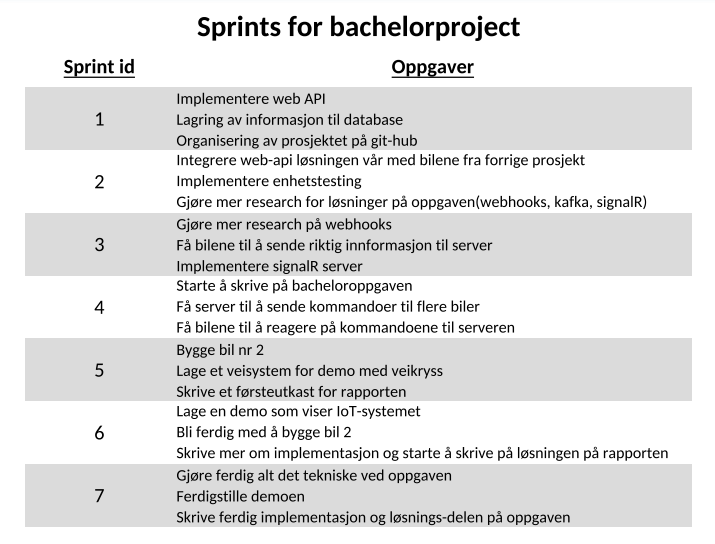
\includegraphics[width=1\linewidth]{figures/Sprint_overview}
	\caption[Sprint overview]{An overview of our sprints. Each sprint lasted 2 weeks. This figure shows the main tasks of each sprint.}
	\label{fig:sprintoverview}
\end{figure}

After a sprint, we would have a sprint retrospective to discuss what went well and what we could have done better. We would also examine if the task assigned in the sprint meetings was finished or needed more work. These meetings helped us reflect over the prior week and adjust accordingly, if necessary. The sessions also helped us determine if we were on track with our initial plan. 
 
In addition to the weekly meetings, we also had daily standups. Daily standups are short meetings, usually lasting around five minutes, where each person answers three questions:
\begin{itemize}
	\item What did the person do last time? 
	\item What is the person going to do today? 
	\item Are there any challenges?
\end{itemize}
We implemented daily standups because it helped our team get on the same page, and it made it easier to plan what each of us had to do that specific day.

Scrum often consists of a team with different roles. As a team of three, we did not feel the necessity to have specified roles because we usually worked together on our projects. However, we alternated on being the scrum master. The scrum master's responsibility is to keep track of the backlog and lead the sprint planning meetings.

\subsection{Kanban as our backlog}
Our implementation of Kanban was to use a Kanban board as the backlog. We used a Kanban board to visualize where a task is in the work process. \figref{fig:kanbanscreenshot} shows an example from our project, with description labels and priority labels:
\begin{figure}[h!]
	\centering
	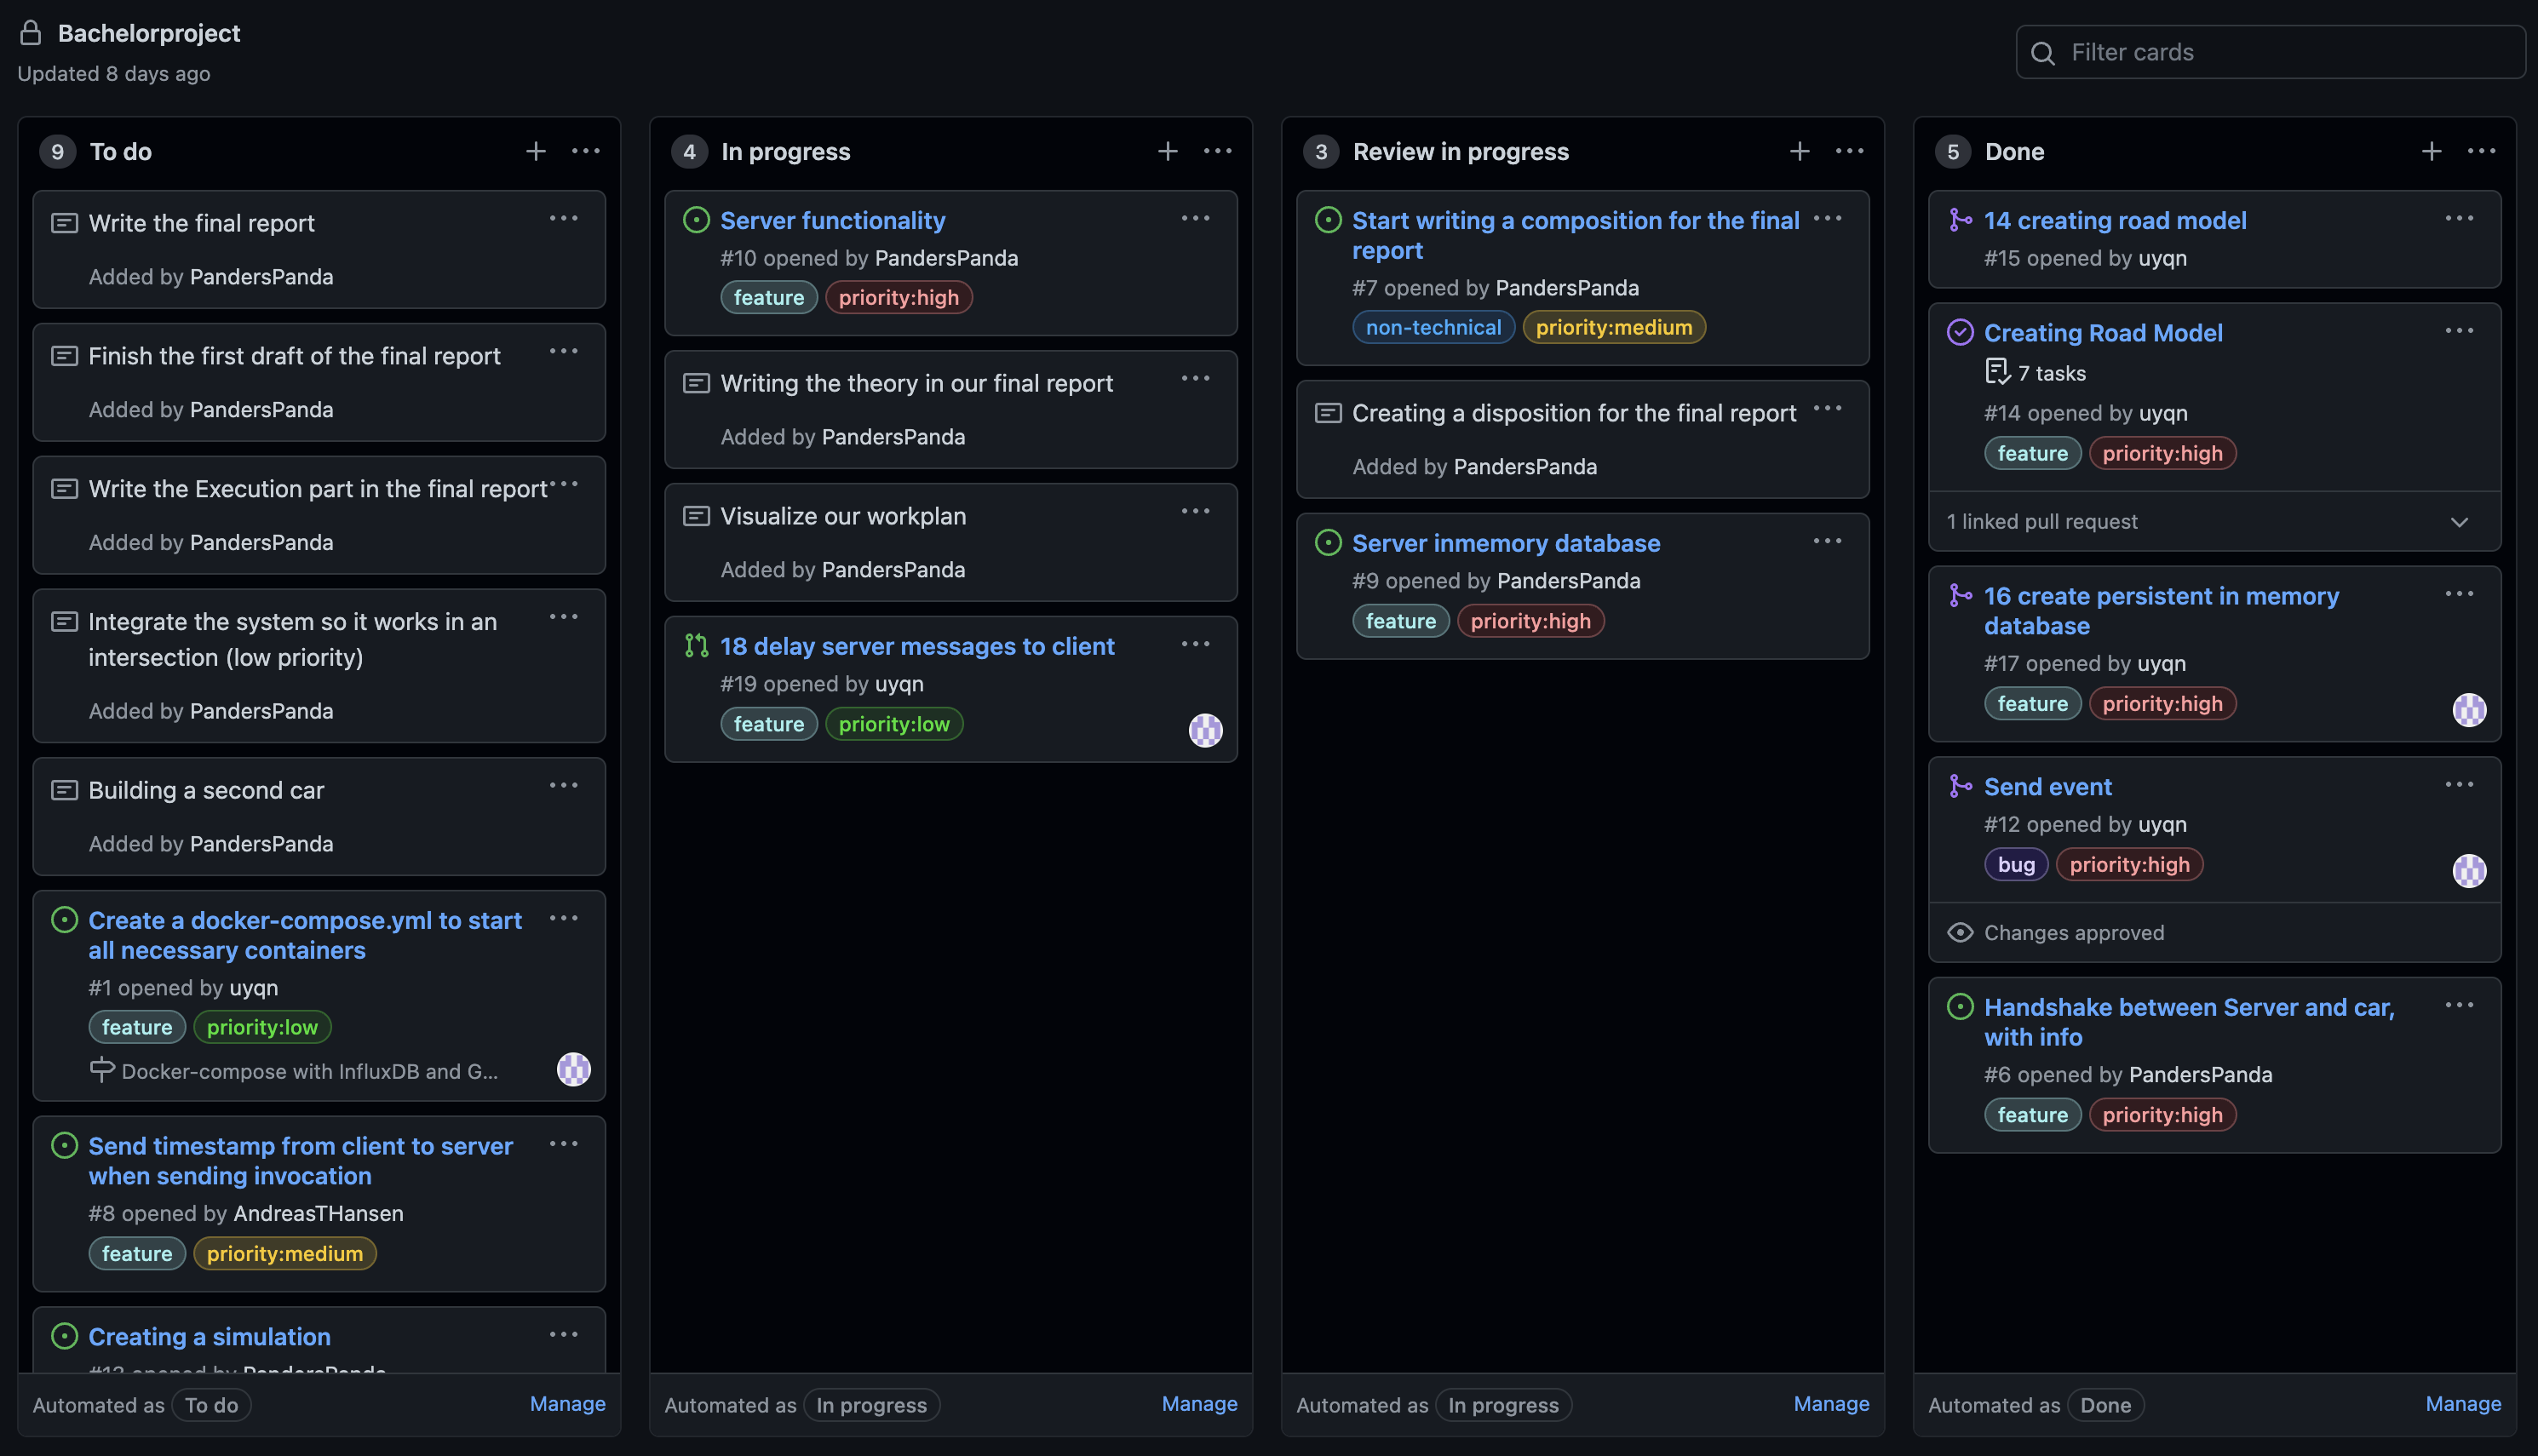
\includegraphics[width=1\linewidth]{figures/kanban_screenshot}
	\caption[kanban screenshot]{Extract of our Kanban board from Github. Each task has a color-coded label representing the priority, and a label to describe the task.}
	\label{fig:kanbanscreenshot}
\end{figure}

We have four columns that represent which phase a task is in. The backlog is the tasks in the to-do column. We dragged it over to the "In progress"-column when we were working on a task. After finishing a task, it went to the "Review in progress"-column, where we reviewed it. If we concluded that the task was finished in the reviewing, it was dragged over to the "Done"-column. Whenever a task is created we tagged it with a high, medium or low to indicate its priority. In addition, to the priority tag, we also gave each task a label; feature, bug, and non-technical to communicate what the task entails. You can also connect the tasks to a specific branch, so the task automatically gets finished when merging the branch into the main branch. The Kanban board was a great tool to see which tasks to choose for our sprints and also keep track of where the tasks were in their process.

However, we did not use the Kanban board throughout the whole process. This is because the backlog was changing a lot, and the Kanban board needed many modifications to be up to date. We figured out that it was more beneficial to focus on one framework, which in our case was Scrum. In addition, we were able to keep track of the tasks by having frequent meetings. 
\section{Tools and technologies}
The circumstances surrounding Covid 19 meant that we could not meet our supervisors in person at the start. Luckily, the group could still meet physically a few times a week. We had to use a wide range of tools for communication. Most restrictions were removed later in the project, but we kept our meetings with our supervisors digital throughout the project. 

\begin{itemize}
	\item Email - Formal communication with supervisors and product owner
	\item Teams - Meetings, and the platform of choice for communicating with the external supervisors on an informal level. 
	\item Zoom - Meetings with our internal supervisor at OsloMet
	\item Facebook Messenger - Communication internally in the group. We used it to send messages to each other when we were not physically together, and to send pictures of code. 
\end{itemize}

The project required us to collaborate while working on different computers, leading to potential overlapping. Therefore, tools that helped us work on the project together were essential. We used the following tools for this purpose:

\begin{itemize}
	\item Git and Github - Version control of choice
	\item Google docs - Used to write our journal and other documents that need to get updated regularly, and to share documents. 
	\item Latex - Used to write reports.
\end{itemize}

We also needed text editors that supported the programming languages that we used. Our solution was created with Python and C\#.
\begin{itemize}
	\item Pycharm - IDE for coding in Python
	\item Visual studio and Rider - IDE for coding in C\#
	\item Thonny - Text editor for coding in Python on Raspberry pi
\end{itemize}

Project planning and documentation were also an important part of the project. The tools we used for the project planning were:

\begin{itemize}
	\item Github project - Kanban board and creating backlog tasks
	\item Excel - Used for visualizing our workplan with tables and a Gantt diagram
\end{itemize}
	\chapter{Implementation}
\section{Process phases}

We chose to split our process into four phases:

\begin{tabular}{l l}
Planning and research phase & week (x-x) \\

API-solution with time series database & week(x-x) \\

Signal-R & week (x-x) \\
Demonstration of our system & week(x-x) 
\end{tabular}
\section{Phase 1 - Planning and research phase}\label{sec:phase1}

After we had gotten in touch with Accenture and spoken with the supervisors and the product owner, the group had to make a few decisions regarding the project's direction.

An important choice for the project was to either build and train an AI model for the vehicles from scratch or use the existing model. Building a new AI model would provide a deeper understanding of the model we could utilize. However, we believed that our project would have the potential to be too similar to the previous project. Also, due to the time constraint, continuing with the existing model was more favorable. Our group also had more prior experience with networking than with Raspberry Pi and AI. We, therefore, chose to use the AI model from the previous project. 

In this phase, we did not have access to the vehicle, nor the code, made by the prior bachelor group. However, there was a need for project planning and research before we could start developing our IoT system. The topics that needed to be researched were:

\begin{itemize}
\item What causes traffic jams and solutions to fix it.
\item IoT-systems and how they function with vehicles.
\item Planning and development methods that will fit our project
\end{itemize}

We also used the pre-project phase to get to know Accenture, their guidelines, and their workspace.

%\subsection{Design thinking workshop}



\subsection{Choice of programming languages}
We chose to implement the client in Python and the server in C\#. The group before us had used Python for their Raspberry Pi vehicle, making Python a natural choice to extend the code from their project. Our group also had experience with networking in Python. Furthermore, the .NET ecosystem has well-developed solutions for creating IoT applications, microservices, and web applications \parencite{dotnet}. We had to write our server in C\#, to take advantage of these solutions. The server needed to be as efficient as possible, and C\# is also considered a fast programming language \parencite{csharp}. We also had some prior knowledge of coding in C\#.

\subsection{Internet of Things}

The Internet Of Things refers to physical objects that communicate using sensors, cameras, software, or other technologies connecting and exchanging data. This communication takes place over the internet or other communication forms. The number of connected IoT devices in the world is increasing, and it is becoming a big part of society \parencite{iot_analytics}. IoT has also been evolving in recent years due to other technologies becoming more accessible, such as machine learning and the 5G network.

IoT projects can, for instance, be applied in climate surveillance systems, energy, or transportation. In this thesis we will explore the possibilities of using IoT in transportation, more specifically in personal automobiles. The convergence of these fields is more commonly known as IoV, Internet of Vehicles. An IoV system is a distributed system for wireless communication and information exchange between vehicles through agreed-upon communication protocols \parencite{chinese_iov}. The system could potentially integrate functionality for dynamic information exchange, vehicle control and smart traffic management. In our thesis, we will explore these possibilities on a small scale.

\subsection{System security}
Security and privacy are important topics for any IoT system. Because these systems gather and work with vast amounts of data, they are naturally prone to be attacked. Moreover, as the systems grow and become more interconnected, with many devices worldwide, the imposed risk of such an attack increases drastically \parencite{iot_risk}. Anonymization of personal data, securing connections, and an intruder detection system are all security measures that require attention. The cars must be able to drive both with or without the system, which is an essential feature of system security. If there is a need for the server to shut down, the cars would need to be able to drive independently of the system. However, this project does not focus on these security measures due to time contraint. 

\subsection{Preventing traffic congestions for a one-lane road}\label{sec:traffic_congestion}

Traffic congestion, also known as traffic jams, is when a long line of vehicles moves slowly or has stopped moving altogether. Traffic jams can create frustration and disrupt nearby local environments with sound and gas emissions \parencite{traffic_congestion_pollution}. Many factors can cause traffic congestion, such as:

poorly designed roads, not wide enough roads, traffic light patterns, and accidents \parencite{traffic_congestion}.

With this in mind, we started by focusing on a simple scenario: when a car drastically reduces its speed or completely stops on a single-lane road.

This scenario will lead to the vehicles behind needing to slow down drastically as well. This phenomenon is called traffic jam shockwave \parencite{traffic_shockwave}. To prevent this, we propose a solution where cars reduce their velocity before they reach the destination of where the shockwave started. For this to happen, a server could keep track of the cars' positions and send information to the vehicles behind, when required. 

We came up with an idea on how the server and cars should interact. First, the car would connect to the server and provide information about its current speed, weight, width, and length. The server would use this information to keep track of all the cars' positions on the road. The cars would send information to the server if their velocity changed. This message would trigger an event on the server where it would command all the cars behind to slow down accordingly. \figref{fig:diagramfirst} shows a flow chart of a potential simulation of this solution:

\begin{figure}[h!]
	\centering
	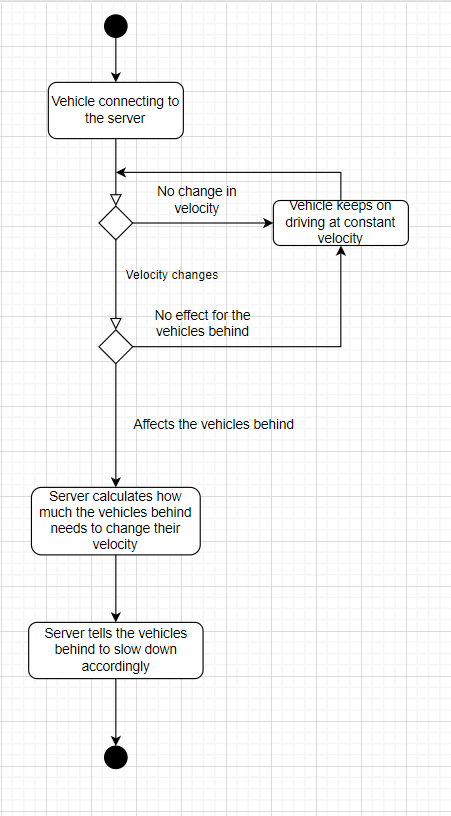
\includegraphics[width=0.9\linewidth]{figures/flow_diagram_first}
	\caption[Flow diagram server]{This figure shows the flow diagram of our first proposed solution. }
	\label{fig:diagramfirst}
\end{figure}
\clearpage
%\section{Implementation of Server and Client}
As IoT-systems become more complex, there is a need to structure them in layers. The three fundamental layers to an IoT-system consists of the perception layer, network layer and application layer \parencite[pp. 347-352]{iot_gateway}. In this part we will discuss what our things-layer and network-layer consists of, and explain the theory behind our decisions. 

\subsection{Implementation of Client}
Raspberry Pi is a small single-board desktop computer that is commonly used for IoT-projects. There is an enormous ecosystem of compatible devices that allow these computers to interact with the world in various ways. The organization states that they can be used for everything “from music machines and parent detectors to weather stations and tweeting bird houses with infra-red cameras” \parencite{raspberrypi}.  For our project we have used a Raspberry Pi Model 4, which the previous group used in their project. This is the newest and fastest model, which makes our test results as accurate as possible.  

The perception layer is responsible for perceiving the world, and creating data for the network layer to collect and deliver \parencite[pp. 8-9]{iot_platforms}. Devices that contribute to this are, for example, Global Positioning Systems(GPS), cameras and sensors. The raspberry-pi models we worked with utilizes both a camera and a range detection sensor that gets processed by the image recognition algorithm running on the machine. These vehicles play the role of client in our system, as they connect to the server. 

The requirements for our client was that it needed to be able to take in commands from the server and respond correctly to those commands. In addition, they had to be able to act by themselves if they were not connected to the server. For that to happen the vehicles had to send their size, position and velocity to the server when they connected initially. The server also needs to send their velocity and position to the server at a frequent rate so that the server can keep track of that information.
\subsection{Implementation of Server}
The network-layer of an IoT-system is responsible for transferring data collected by the things-layer \parencite[pp. 8-9]{iot_platforms}. In our project this is done by a centralized server that is connected to all the clients. 

The task required the client, which in our case is the cars, to receive the commands from the server. The group prior had made it such as the car made decisions based on its AI. The AI used picture recognition which could recognize speed limit signs and stop signs. The cars were also programmed to follow a path. Furthermore we needed a server which could send commands to the clients at a frequent rate, based on the information given by the clients. The server’s commands need to overwrite the AI that is already on the vehicles.

Here are some requirements needed for the server:
\begin{itemize}
	\item Needs to be able to send messages to all clients simultaneously, or a specific group of clients.
	\item Handle increasing traffic
	\item Little to no delay
	\item Two way communication between server and client
\end{itemize}

We initially coded a server by using API. The server was able to receive information from the clients, but for the cars to receive information from the server, they had to host their own servers. The car’s main priority should be calculating decisions based on their AI, not hosting a server. It would also be harder to add a server to the code from the previous group. We therefore thought of some other solutions. 

Websockets provides a two way communication over a single tcp-connection. This means that both the server and client can send and receive messages from each other. They also allow for a better efficiency than REST API because they do not require the request/response overhead for each message that is sent and received. This solved the issue we previously had with the solo API-solution.

ASP.NET Core Signal R is an open source library that simplifies adding real-time web functionality to apps (Microsoft, 2022). It supports websockets as a real time communication which is perfect for a two way communication. Signal R is often used in games, social networks and gps-apps where information to the clients are needed instantly. It also scales with increasing traffic. Signal R uses hubs where servers and clients communicate with each other. Hubs allows servers and clients to call methods on eachother. Since the server needs to send the cars commands this is perfect for our Iot-system.

The server needed some specific functionalities in correlation with the problem statement stated earlier. We did some research on what caused traffic jams and chose two problems which our server would focus on solving:

\begin{itemize}
	\item Delayed reaction times when people stop and accelerate 
	\item Increased traffic flow in intersections
\end{itemize}

The first point happens when a car changes velocity. Therefore the server has to check if any car’s have changed their velocity. If yes, the server needs to send a command to all the car’s behind a certain distance of the car that changed their velocity.  The distance will be calculated by the server based on the change of velocity. The command sent out to the car’s behind will be to change velocity based on distance to the car that changed their velocity and the amount of changed velocity.

To increase traffic flow in intersections we can have the server work as some traffic lights. The server can check if cars are closing in on the intersection’s position and give one lane the green light and the other the red light. The lights will depend on which car’s come first. The difference between a server doing this and a traffic light system is that the server can tell the vehicles to slow down before the intersection, making the traffic flow smoother.
%\section{Implementation of simulation}
To show that the solution was reaching the requirements we needed to create a demonstration. A demonstration was also an important part of testing the functionalities of the IoT-system. There were two options which were viable in this case. The first one was to create a virtual simulation using unity or another graphic-program. The other option was to build a physical demonstration with two or more cars. We chose to implement a physical demonstration with two cars. This was because we already had one car finished by the previous group. In addition it was more beneficial for Accenture with a physical demo since they can show it at exhibits.
\begin{itemize}
	\item That the server can turn off and the cars would still drive on their own.
	\item Cars communicating through the server and acing based on the server’s decisions
	\item Scalability to the real world
\end{itemize}
First we built the server with only one single lane road in mind. With this solution the potential of showing off the functionalities of the IoT-system was low. We could potentially have shown that if a car in front slows down, the car behind also slows down. This would show that the system could prevent some traffic, but only in a specific scenario. However we wanted to show that the IoT system could work in more than just one single-lane road. We therefore chose to try to emulate an intersection in the physical demo.

For a physical demo to work we needed to build another car. Luckily the previous group had documented their work and we could follow their process from their final report. We also had the parts provided to us. However we were unable to get the full functionality of the second car since the TPU accelerator used by the previous group was unavailable. The TPU accelerator provided the car with the processing power needed for the AI. This meant that the car was built without the camera. But this had a minor effect on our demo since the other car was fully functional without the system. We solved this problem by letting the server do the decision making for the car with less functionality.

We also needed to emulate a road system which contained the intersection we were going to demonstrate in the demo. Since the AI had not trained to recognize intersections yet we had to code a road system into our server that contained roads, lanes and intersections. We then had to build a physical intersection for our cars with tape that correlates with the emulated intersection. 

\subsection{Calibration of the cars}
When the server, vehicles and client were implemented, and the second vehicle built, we did some testing to figure out how the car’s behaved when given directions by the server. In this test the vehicles were given a specific velocity and driving distance by the server. When the vehicles arrived at their destination the server would tell them to stop. The car’s drove in a straight line.

The vehicles were able to send information, and respond correctly to the servers commands. We also observed that the vehicles drove a different length for each velocity given even though the length was the same. This is because the velocity given to the vehicles is the amount of power going into the car’s motors, not the actual velocity of the car’s. We wanted the demo to be accurate so our group did some further testing where we wrote down the results. 

\begin{table}
	\begin{center}
		\begin{tabular}{rrrr}
			\hline
			Power (?) & Length (cm) & Time (s) & Velocity (cm/s) \\
			\hline
			40 & 467 & 8.98 & 52.00 \\
			50 & 425 & 7.28 & 58.38 \\
			60 & 400 & 6.06 & 66.01 \\
			70 & 357 & 5.18 & 68.92 \\
			80 & 325 & 4.49 & 72.32 \\
			90 & 314 & 4.03 & 77.92 \\
			100 & 286 & 3.62 & 79.01 \\
			\hline
		\end{tabular}
		\caption{Test text}
	\end{center}
\end{table}

The data Power was the velocity given by the server. Velocity was the actual velocity in our testing, which is length divided by time. As you can see the velocity was not the same as the power. We then made a graph to visualize the two values. The $y$-axis was the velocity while the $x$-axis is the power.

\begin{figure}[h!]
	\caption{Graph of velocity as a function of power}
\end{figure}

We observed that the correlation between power and velocity seemed linear. This means we could make a specific formula that describes the correlation between the two values. We used linear regression to figure out this formula:

\begin{figure}[h!]
	\caption{Graph of velocity as a function of power with linear regression}
\end{figure}

The formula we ended up with was as follows: $P = 0.4516v + 36.189$, where $P$ is power and $v$ is velocity, with a mean square error of $R^2=0.9653$. When we coded the formula into the vehicles we did another set of testing. We observed that the vehicles drove more or less the same distance for each power given. If we wanted an even more accurate formula we could have tuned the formula with the test results from our new test. Although the results were not hundred percent accurate, we concluded it was accurate enough for our demonstration. 

To test the solution we have worked on, we made a physical demonstration with two cars that meet at an intersection, as part of the product documentation. We want to test that a combination of a centralized communication system and artificial intelligence can improve traffic flow. What we wanted to observe was if the velocity of the vehicles were not drasticly changed and therefore not distrupting the traffic flow.


%\subsection{System security}
Security and privacy are important topics for any IoT system. Because these systems gather and work with vast amounts of data, they are naturally prone to be attacked. Moreover, as the systems grow and become more interconnected, with many devices worldwide, the imposed risk of such an attack increases drastically \parencite{iot_risk}. Anonymization of personal data, securing connections, and an intruder detection system are all security measures that require attention. The cars must be able to drive both with or without the system, which is an essential feature of system security. If there is a need for the server to shut down, the cars would need to be able to drive independently of the system. However, this project does not focus on these security measures due to time contraint. 
\section{Phase 2: REST API}\label{phase2}
The aim of the project was to connect Raspberry Pi devices to a system. Thus, the group decided that the best way to establish this connection was to implement a RESTful API on the server. In addition, the question on how the data should be stored was also arises during this phase.

\emph{Representational state transfer} (REST) \emph{application programming interface} (API) provides a way for client and server to establish communication through \emph{hypertext transfer protocol} (HTTP). Using a REST API clients can send requests to a server to perform standard CRUD (create, read, update and delete) operations on a database \parencite{rest_api}.

Due to the time sensitivity of the application we are trying to build, it was therefore necessary to choose an appropriate type of database for our system. In this case, we chose to incorporate the time series database. InfluxDB is a time series database created by InfluxData. It provides a SQL-like syntax for querying resources that is quick and scalable, and most importantly free. Moreover, InfluxDB client library, using the influxDB v2 API, provides both ease of install and use for a multitude of langauages \parencite{influxdb}.

During this phase the group implemented a standard REST API server with C\# with the idea that the Raspberry Pi vehicles should exchange information on its velocity, acceleration and position to the server. Client should first POST itself to the server. The server will then add the vehicle to the influxDB to keep track of the vehicle's information. Then, the vehicle should be able to perform a GET request to the server to retrieve its information.

The client at this phase would be able to send a PATCH request to the server in order to update its information. In addition, the server will add a new entry into the database whenever it receives this request. The idea was that the client and server would be able to continuously communicate to each other such that the server could determine the behaviour of all connected clients.

However, a RESTful API server were not able to perform all its required task that the group wanted the server to do. Firstly, the server were only able to communicate with one client at the time, i.e. the client that sends a request. What the group wanted at this stage was that based on a request the server should also be able to send its own request to all the other clients. In order to acheive this, the server had to send an unprompted response to other clients that is not requesting a resource from the server, which was not possible with our current architecture.

A new solution had to be in place in order to achieve our goal. Other solutions were proposed during this stage.

\subsubsection*{Long polling}
Polling is the idea that the server pushes resources to the client. There are mainly two types of polling; short- and long polling. 

In short polling, a client requests a resource from the server and the server responds with nothing if the resrouce is not available. The client will then send a new request in a short amount of time and the cycles repeats until the client receives the resource it has requested.

Long polling is similar to short polling, however, the server does not send anything back before the resource is available. That is, the client sends a request to the server and the server is holding this request until it has a response available to the client. In our case, we wanted every client to perform a GET request to the server on a seperate thread and instruct the server to hold onto this request until it had further instructions to the requesting client.

However, implementing a method on the server to block the response introduced more complication to the project. Also, with the asynchronous nature of the controllers implemented on the server it would also mean that the server will consume a lot of the processor which also means that the performance of the server will be heavily deteriorated.

\subsubsection*{Implement REST API on the client}
Another solution was to implement the client itself as a REST API server on its own. However, in order to achieve this, each client needed to also send the server its host and port information to the server. Also, the server has to be implemented as a client in order to connect to the vehicles.

\subsubsection{Webhooks}
Webhooks, according to \cite{webhooks}, is a user-defined callback over HTTP. In our case, implementing webhooks to post notifications on clients based on events sent to the server. This was a good contender to solve our issue. However, implementing webhooks includes extensive research into a system the group had never heard of, in addition to scarce information on how to create such a system. The group decided that the time constraint of this project did not justify the time it would take to implement such a system.

\section{Phase 3 - Websocket with SignalR}\label{phase3}
After extensive research on how to solve the two-way communication discussed in \secref{phase2}, the group agreed that WebSockets would be an excellent solution to our problem. Using WebSockets, both client and server can transfer data whenever they see fit. However, \cite{microsoft_websockets} discourages developers from implementing raw WebSockets for most applications and recommends using SignalR instead.

ASP.NET SignalR is a library that at the top layer provides real-time communication using WebSockets while also providing other transport methods such as long-polling as fallback \parencite{microsoft_signalr}. Furthermore, SignalR API supports \emph{remote procedure calls} (RPC) using hubs, meaning we can invoke subroutines on the client from the server and vice versa \parencite{microsoft_signalr}.

As a result of the failure to attain the result we wanted with REST API and InfluxDB, as discussed in \secref{phase2}, we decided to implement SignalR without InfluxDB on our server instead. First, set up an echo server using SignalR while simultaneously implementing the client code. The client code had to be implemented independently of the Raspberry Pi code. Because our goal was to create a communication module that is reusable through inheritance for other devices, e.g., traffic lights, should it be required to set up a new hub with other devices.

After successfully implementing all the necessary methods on the client, the vehicle class representing the Raspberry Pi device became our next priority. By inheriting the client class, the vehicle class also inherits its ability to connect, listen and send data to the server. Furthermore, the client can also subscribe to events that the server can trigger using RPC.

\subsection{Implementation of traffic on a single lane}
After witnessing a successful connection between the Raspberry Pi vehicle and our SignalR server, we started to implement the necessary functionality on the server. We started with the simple scenario described in \secref{sec:traffic_congestion}. The client will inform the server whenever its velocity has changed. Then, the server will relay this change to every other vehicle behind it on the same road and adjust their velocities accordingly. This server functionality also depends on the continuous monitoring of each vehicle's position. Thus, raising a new issue on how the vehicle information should be stored.

InfluxDB could, in theory, be used to store the vehicle's position; however, since the position is constantly changing, it would require the server to read and write on the database continuously. Hence, the group concluded that this would potentially impact latency on the server. Thus, we unanimously determined that a live-in-memory database storing vehicles in lists would be preferable. With simple mathematics, the server could recalculate the vehicle's position based on its previous velocity and a stopwatch whenever it retrieves the information about a vehicle instead.

We then determined to show the product owner from Accenture what we had been working on, thus inviting him and the external supervisor to the next meeting. This short demonstration consisted of running multiple clients with the server to simulate how multiple vehicles would behave with the intervention of our server. The simulation successfully demonstrated that vehicles were able to adjust their velocities in order to prevent the shockwave phenomena described in \secref{sec:traffic_congestion}, and we received positive feedback. However, our supervisors challenged us to extend our concept and make our solution more complex. They believed implementing an intersection where multiple cars meet could show more advanced traffic management. They believed implementing an intersection where multiple cars meet could show more advanced traffic management.

\subsection{Extending the concept to a more complex scenario - traffic on an intersection}
Expanding further on the concept, new functionalities on the SignalR server were developed to handle vehicles approaching an intersection. With a more complex topology, expanding the database to account for the new road network is also required. Consequently, roads and intersections became required additions to our solution. Furthermore, the vehicle model on the serverside is now also composed of a route planner to represent what it means to be approaching an intersection.

With these improvements and new functionalities, the server can command the clients to adjust their velocity to avoid collisions between vehicles approaching an intersection simultaneously. By reducing the velocity of some vehicles, it also became apparent that traffic flow is improved, in contrast to stopping a vehicle.
%\subsection{System security}
Security and privacy are important topics for any IoT system. Because these systems gather and work with vast amounts of data, they are naturally prone to be attacked. Moreover, as the systems grow and become more interconnected, with many devices worldwide, the imposed risk of such an attack increases drastically \parencite{iot_risk}. Anonymization of personal data, securing connections, and an intruder detection system are all security measures that require attention. The cars must be able to drive both with or without the system, which is an essential feature of system security. If there is a need for the server to shut down, the cars would need to be able to drive independently of the system. However, this project does not focus on these security measures due to time contraint. 
\section{Phase 4 - Making a demo}

At this point in the development we were sure about what kind of situation we wanted to simulate to make a satisfying product for Accenture, and to answer the problem statement we had decided on. Following the work requirements we now needed to make a demonstration that showed how the system worked. At this point we also decided that we wanted to make a physical demonstration instead of making a digital simulation, although this was a solution that would take less effort and still be a valid solution. At the start of this work phase we had started to consider making only a digital simulation, but after a meeting with our external supervisors at Accenture, in which we were advised that a physical demonstration was more in line with Accenture's goals for the project, we finally decided to make a physical demonstration. 

\subsection{Building a new car}
The previous group had only built one car for their project. Consequently, we needed to build a new car to show a situation where two cars meet at an intersection. Luckily, Accenture kept a box of unused components from the previous group. However, we only had one TPU, the Coral Usb Accelerator. The TPU is an essential component for giving extra processing power to the computer, and it was necessary to run the artificial intelligence the previous group had used \parencite{prev_project}. 

Without this accelerator, we could not run the artificial intelligence the previous group had incorporated into their solution due to the global chip shortage caused by the Covid pandemic; the accelerator was unavailable to purchase anywhere. As a result, the new car's camera and distance measuring sensor were absent. Not having two cars that utilized artificial intelligence could be a challenge. One of the required features of our solution was that the cars should be able to drive using the AI when a server connection was unavailable, as per described in \secref{sec:goals}. We decided that as long as we had one car that could navigate traffic independent of the server, the other car could drive solely on commands given by the server. With the components and the product documentation of the previous project \secref{sec:goals}, we were able to build a copy of the car as seen in \figref{fig:twocars}.

\begin{figure}[h!]
	\centering
	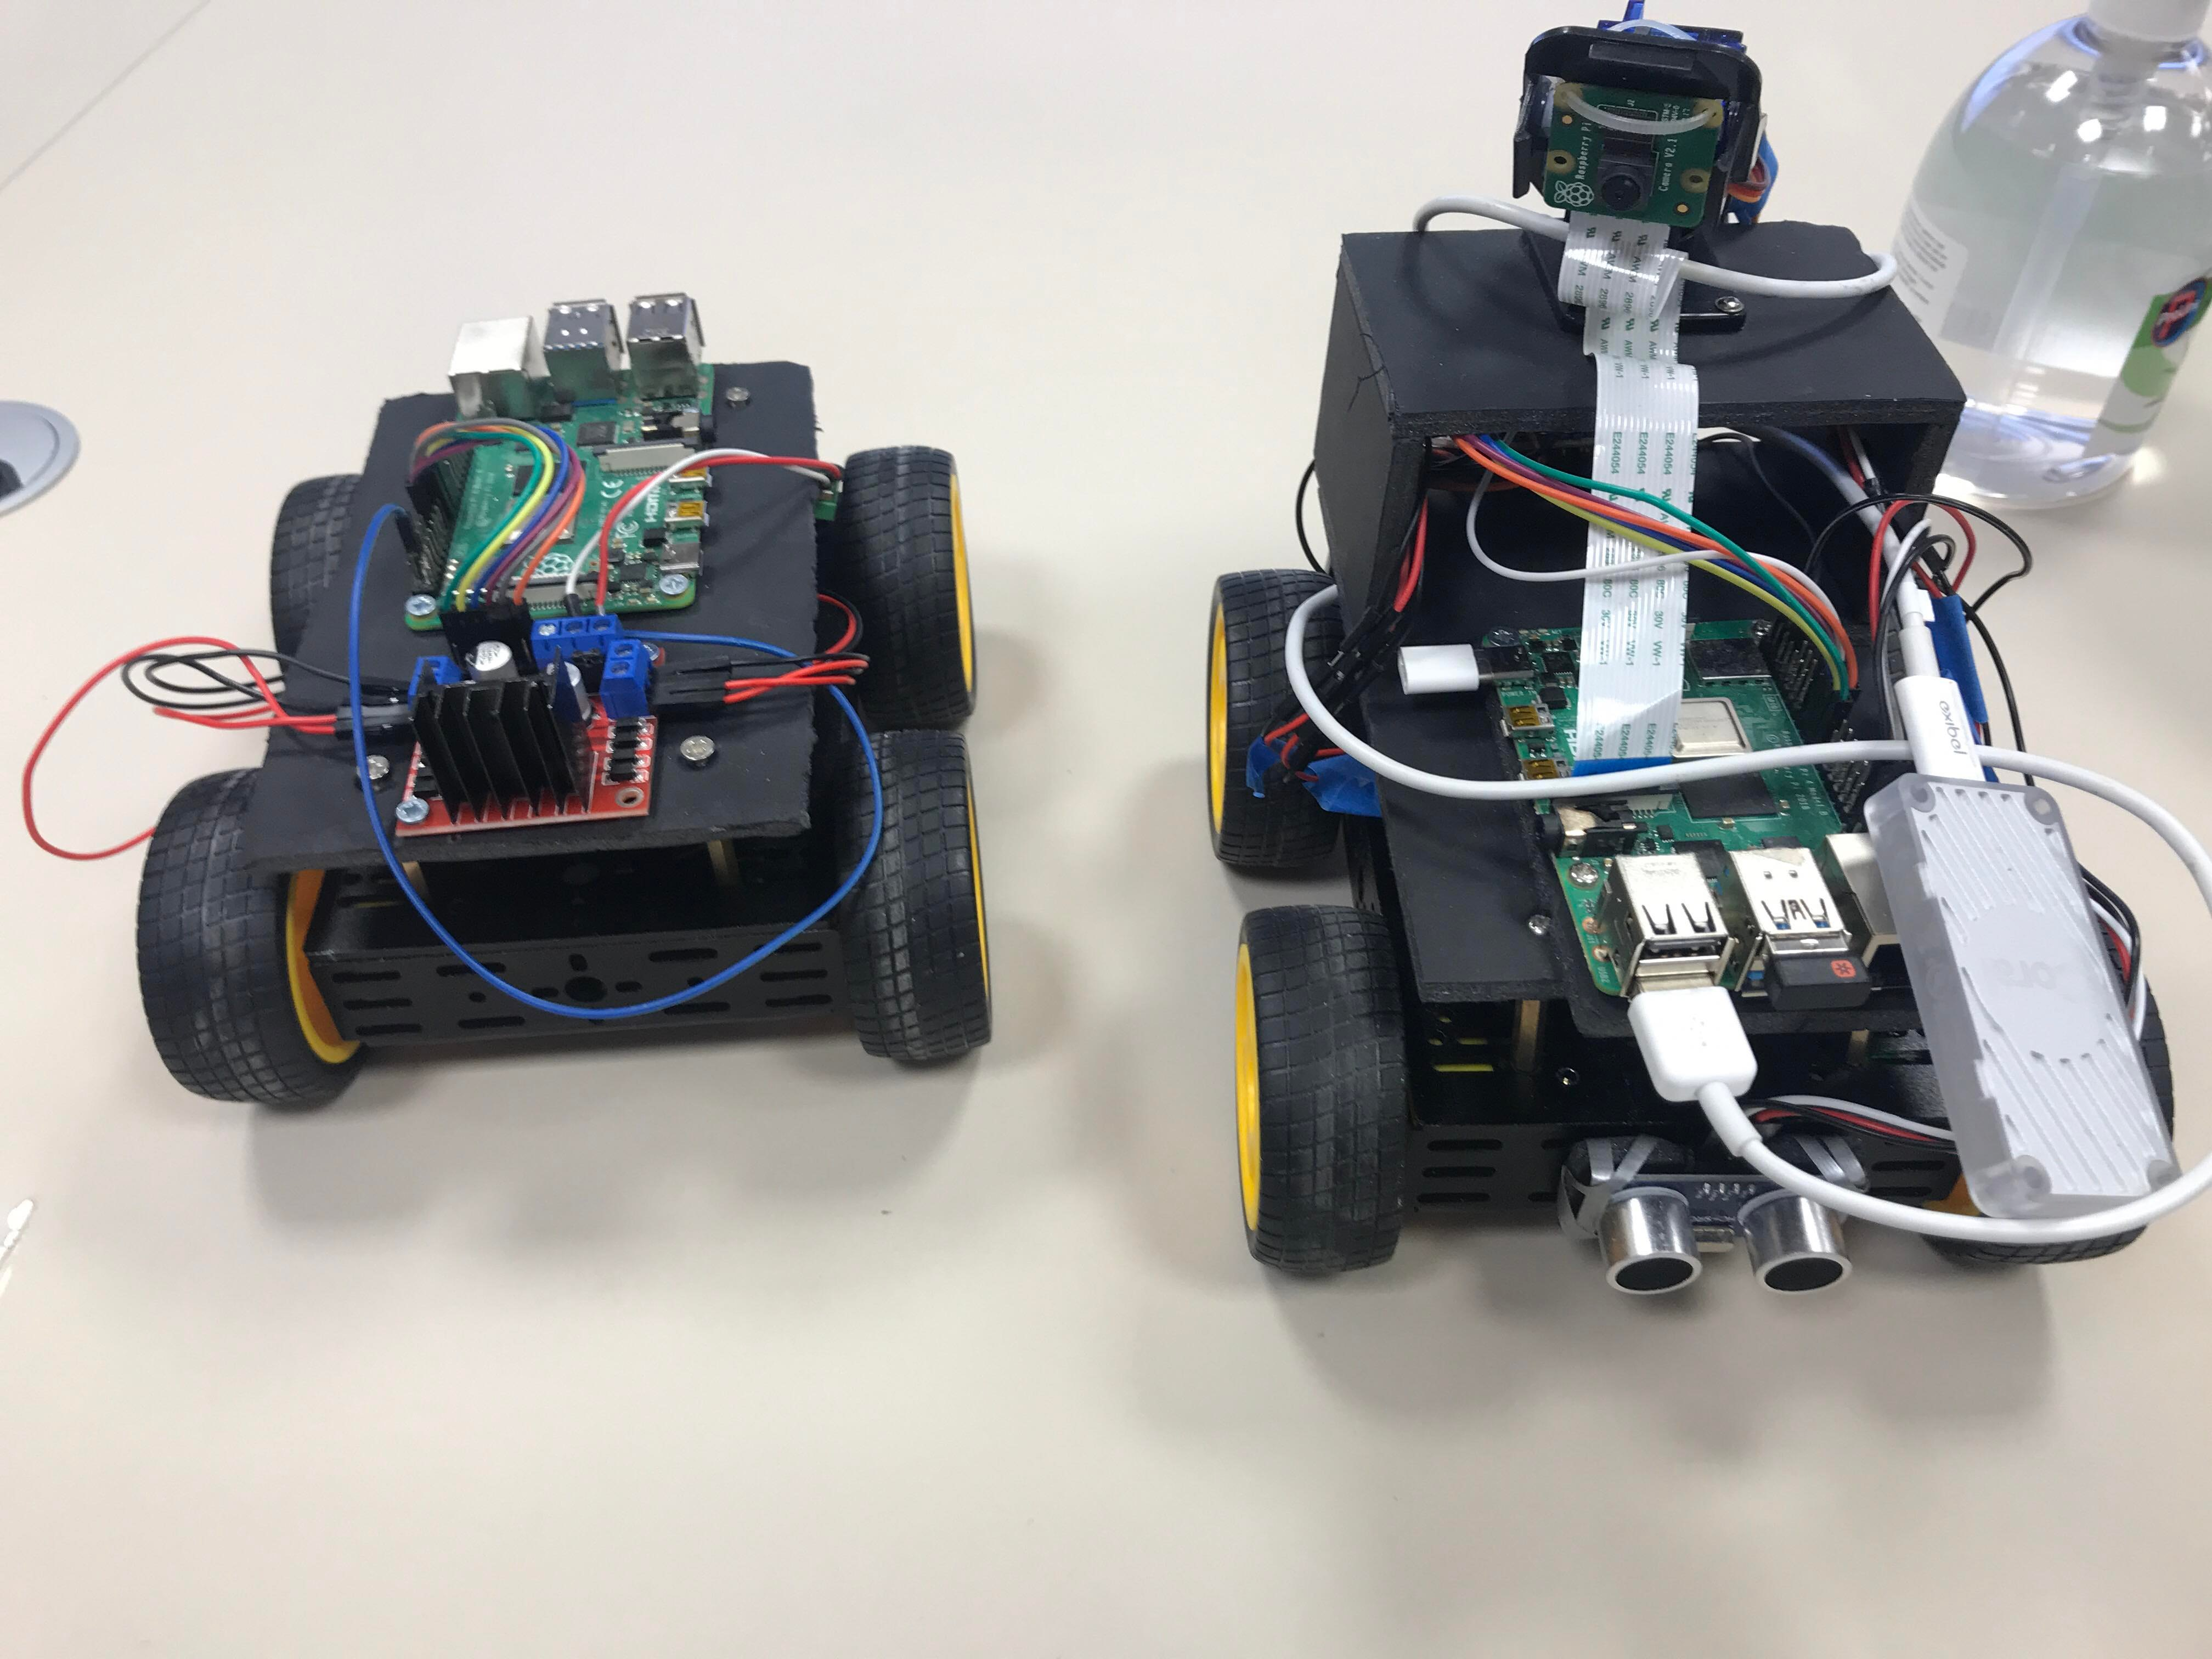
\includegraphics[width=0.9\linewidth]{figures/two_cars}
	\caption{Photo of the two cars we built. To the left is the car without a camera. To the right is the car with a camera on top and a Coral USB Accelerator Edge TPU. This car can take advantage of the onboard AI.}
	\label{fig:twocars}
\end{figure}




\subsection{Calibration of the cars}
When the server, vehicles and client were implemented, and the second vehicle built, we did some testing to figure out how the car’s behaved when given directions by the server. In this test the vehicles were given a specific velocity and driving distance by the server. When the vehicles arrived at their destination the server would tell them to stop. The car’s drove in a straight line.

The vehicles were able to send information, and respond correctly to the servers commands. We also observed that the vehicles drove a different length for each velocity given even though the length was the same. This is because the velocity given to the vehicles is the amount of power going into the car’s motors, not the actual velocity of the car’s. We wanted the demo to be accurate so our group did some further testing where we wrote down the results. 

\begin{table}
	\begin{center}
		\begin{tabular}{rrrr}
			\hline
			Power (?) & Length (cm) & Time (s) & Velocity (cm/s) \\
			\hline
			40 & 467 & 8.98 & 52.00 \\
			50 & 425 & 7.28 & 58.38 \\
			60 & 400 & 6.06 & 66.01 \\
			70 & 357 & 5.18 & 68.92 \\
			80 & 325 & 4.49 & 72.32 \\
			90 & 314 & 4.03 & 77.92 \\
			100 & 286 & 3.62 & 79.01 \\
			\hline
		\end{tabular}
		\caption{Test text}
	\end{center}
\end{table}

The data Power was the velocity given by the server. Velocity was the actual velocity in our testing, which is length divided by time. As you can see the velocity was not the same as the power. We then made a graph to visualize the two values. The $y$-axis was the velocity while the $x$-axis is the power.

\begin{figure}[h!]
	\caption{Graph of velocity as a function of power}
\end{figure}

We observed that the correlation between power and velocity seemed linear. This means we could make a specific formula that describes the correlation between the two values. We used linear regression to figure out this formula:

\begin{figure}[h!]
	\caption{Graph of velocity as a function of power with linear regression}
\end{figure}

The formula we ended up with was as follows: $P = 0.4516v + 36.189$, where $P$ is power and $v$ is velocity, with a mean square error of $R^2=0.9653$. When we coded the formula into the vehicles we did another set of testing. We observed that the vehicles drove more or less the same distance for each power given. If we wanted an even more accurate formula we could have tuned the formula with the test results from our new test. Although the results were not hundred percent accurate, we concluded it was accurate enough for our demonstration. 

To test the solution we have worked on, we made a physical demonstration with two cars that meet at an intersection, as part of the product documentation. We want to test that a combination of a centralized communication system and artificial intelligence can improve traffic flow. What we wanted to observe was if the velocity of the vehicles were not drasticly changed and therefore not distrupting the traffic flow.


\subsection{Construction of semi physical demonstration}\label{sec:demo}
We wanted to test that a centralized communication system and artificial intelligence could improve traffic flow. In order to test the solution, we made a semi physical simulation where two cars approach an intersection simultaneously. We wanted to observe if the velocity of the vehicles were not drastically changed and, therefore, decreased shockwave described in \secref{sec:traffic_congestion}.

We found a space at Accenture that was big enough to build the track. The power input on the Raspberry Pi vehicles is limited to between 40 and 100 units. Since the server will adjust the vehicle's speed to avoid a collision, the intersection was required to be at least 130cm away from the starting point to prevent the server from adjusting speed outside the equivalent power limit. Furthermore, the server prevents cars from driving before at least two vehicles have established a connection. Hence, both vehicles will start their journey simultaneously. We also placed the vehicles at the same distance from the intersection on their respective roads. Given these initial conditions, both vehicles are supposed to collide without the server's intervention. We also made the server log the velocity sent to the cars to track how much the cars' velocities changed.

Making the demo one hundred percent accurate was not possible in our circumstances due to the limitations of the Raspberry Pi. Furthermore, the vehicles were not able to receive the messages simultaneously. Consequently, this meant that they could start with a minor time difference. Another factor was that the trajectory of the vehicles was not always straight. However, we were able to get a consistent demo with enough margins. \figref{fig:crashdemo} shows an example of a collision during a test demonstration.

\begin{figure}[h!]
	\centering
	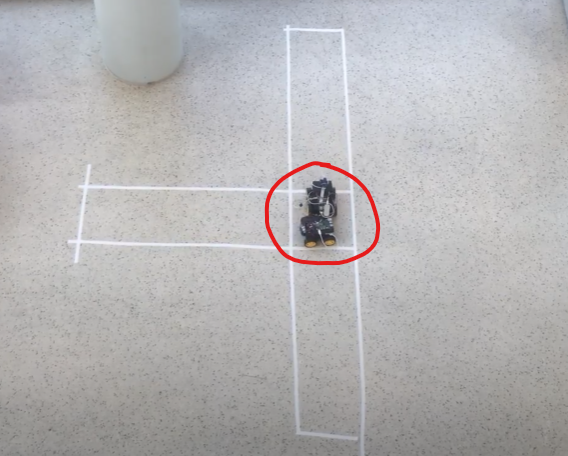
\includegraphics[width=1\linewidth]{figures/demo_crash}
	\caption{Here, we can observe the two cars colliding in the intersection. One of the cars started about 5 centimeters further behind the other car and started a few milliseconds later, resulting in a collision. Meanwhile, the server assumed they started simultaneously at the same distance from the intersection.}
	\label{fig:crashdemo}
\end{figure}

Furthermore, the server did not account for the lengths of the vehicles during its calculations. After we introduced the length of the vehicles and buffer zone, we were able to get a consistent semi-physical demonstration.

When both vehicles had connected to the server, the cars would drive with an initial speed of 80 cm/s, the upper limit of the Raspberry Pi. Not long after they started to drive, the server recognized the cars approaching the intersection. The server calculates using the car's velocity, position, and length. Then the server calculates which car has to slow down and how much the car needs to slow down to avoid a collision, in this case, to 55 cm/s. After the other car has supposedly passed the intersection, the car that slowed down gets told by the server to speed its velocity back to 80 cm/s. \figref{fig:successdemo} is a snapshot of a successful test demo.

\begin{figure}[h!]
	\centering
	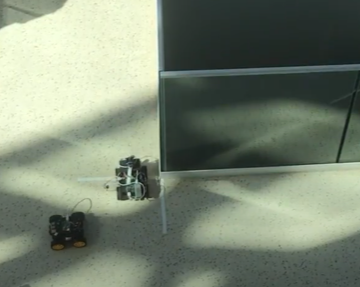
\includegraphics[width=1\linewidth]{figures/succsess_demo}
	\caption[Successful demo]{Here is a snipped from a successful demo. The car to the left has just passed the intersection, marked as a square with white tape. The car furthest up is, therefore, about to adjust back to its original velocity. Here we can observe that the server prevents a collision.}
	\label{fig:successdemo}
\end{figure}
%\input{chapters/sections/subsections/building_road_model}
%\input{chapters/sections/subsections/simulating_situation}


\chapter{Conclusion}
\section{Results}
In regards to the problem statement in \secref{sec:problem_statement} and the goals for this project discussed in \secref{sec:goals}, we have been able to successfully create a centralized system that communicates that can communicate with autonomous vehicles. A significant change in velocity can lead to a disruption of traffic flow, as discussed in \secref{sec:traffic_congestion}. Through multiple semi-physical demonstrations discussed in \secref{sec:demo}, it was apparent that the server was able to contribute to an improved traffic flow by preemptively reducing vehicles' to the necessary speed to prevent collisions. Even though this project did only account for scenarios involving intersections, it is also from the exploration done throughout this project that autonomous vehicles, together with a centralized system, can be the answer for improving traffic flow in the future.

Furthermore, we received positive feedback after showing our supervisors and product-owner video snippets of the conducted demonstrations. Additionally, the product owner confirmed that our results adhered to the requirements set by Accenture.

\subsection{Real world scenario}

If we compare the data from the semi physical demonstration to a real world cenario were instead of 80 cm/h the cars would drive in 80 km/h prior to an intersection. In the real world, one of the cars would have to stop before a traffic light while the other could drive past the intersection. This would lead to a velocity change from 80 km/h to 0. In our scenario the car would only have to slow down to 55 km/h.

However there are more factors to consider in a real world scenario such as: curved roads, human mistakes and animals jumping onto the road.
\subsection{Possible improvements}
All the features in the MoSCoW method from \secref{sec:moscow_method}, "could have" to "won't have this time" are features for a future project, either for Accenture to improve or for a future bachelor project. Although it fulfilled the product requirements given by Accenture, there is room for improvement. For example, with the accuracy of the demo, specifically by doing more calibration tests and making a more accurate formula than we were able to produce (see \hyperref[eq:vprelationship]{equation \eqref{eq:vprelationship}}). Furthermore, changing the wheels and installing an edge TPU to exploit the existing AI model will result in a more predictable trajectory of the vehicles.

Our demo only contains two cars, but our server supports scenarios with multiple cars. There are also possibilities to connect other devices to the server, for example, traffic lights. However, there are no specific functionalities for other IoT devices on the server. Scaling the IoT system for functionalities with other IoT devices is a task for future development. Adding roads and making a more complex road system would also be a task for future development.

As mentioned, we made a semi-physical simulation. However, a virtual simulation would potentially yield more data for research while also exploring other more complex road configurations.

Due to this project's time constraints, we, for instance, did not integrate machine learning with our server. Integrating machine learning on the server could expand its different capabilities and make the project more scalable and applicable to a broader range of scenarios. Such integration is deemed valuable for the further extension of this project.

Making a viable product in the real world is a long way ahead and will require a lot more testing and implementation on a bigger scale. With the rise in availability of self-driving vehicles and the 5G network, there could be a possibility of IoT systems managing traffic. We explored the posibility of implementing multiple servers, each  having responsibility for their own geographical area, or an entire road. This follows the edge computing architecture, which is popular in IoT systems and describes distributed network devices that communicate to one centralized server through ``edge'' devices \parencite[pp 149]{iot_platforms}. We did not implement this in our program, but it was one of our main ideas for how we would scale the system to implement more roads.

Finally, we hope that our testing and research can be of value towards realizing autonomous cars and traffic management on such a scale.

\section{Further discussions}
In addition to implementing the program, we also had discussions regarding the viability of the program. Here we will discuss our process and how such an IoT system would apply to the real world. We will use our data and some research to reflect the usability of an IoT system where self-driving cars can communicate with each other.

\subsection{Self evaluation}
As mentioned earlier in \secref{sec:dev_method}, we took inspiration from two agile frameworks: Scrum and Kanban, but chose to lean more towards scrum in the end. The use of Scrum helped us reach our goals. However, we could have included our external supervisors more in the Scrum process in hindsight. We could have done this by including them in sprint retrospective meetings and discussing what our following sprint goals should have been together.

The IoT system can handle more vehicles, but the road model does not fully support functionalities for having more intersections than we currently have in our demonstration. Because of the time constraint, we also found it challenging to focus on scalability. Hence, we instead focused on getting a working demonstration.  

One challenge was that our group could not meet as much as we had wished because of work. However, all the requirements in the MosCoW analysis (\figref{fig:moscowmethod}) were reached except for the features in the "can have" section. All in all, the group was satisfied with the process.

\input{chapters/sections/subsections/educational_value}
\section{Further work}
How to implement self-driving in society in the best way is a question that will take a long time to answer. Through our work with this proof-of-concept we believe we have made an addition to this discussion. Due to time constraints, we have chosen not to implement some features that would make the product work in a more complex environment. These features could be explored if this project were to be further developed. 

\input{chapters/sections/subsections/scalability}
\input{chapters/sections/subsections/extendability_real_world}
\input{chapters/sections/subsections/risk_management}

%	\chapter{Product documentation}
\section{Preface}

The product documentation is a technical description of the product.

The product documentation assumes the reader has some prior knowledge in basic programming.
\section{Program description}

\begin{figure}[h!]
	\centering
	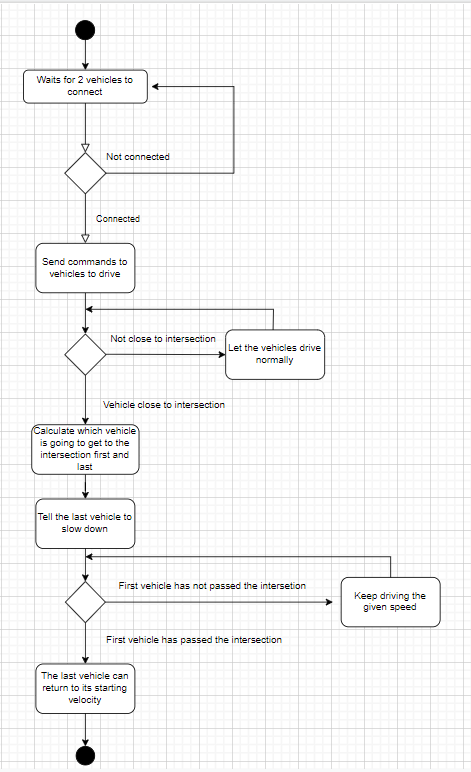
\includegraphics[width=1\linewidth]{figures/Flow_diagram_server}
	\caption[Flow diagram server]{Flow diagram for the server. This diagram specificly shows the flow of the semi physical demonstration.}
	\label{fig:diagramserver}
\end{figure}

The program is an IoT-system were vehicles can communicate with eachother through a server. It constists of a server which has the responsibility for the calculations and decision making, and a client which are the vehicles. The function of the program is to increase traffic flow and prevent traffic congestion. As of now the program can be used in an intersection with two vehicles, but can be scaled to include more vehicles. Here is a diagram that describes the flow of our server in the demonstration:




\clearpage
\section{Adherence to project requirements}
Our solution adheres to the requirements Accenture set for us. Our prototype cars can work both with, and without being connected to a server. The server can handle multiple connections and adjust trafic based on the situation on the road. Through er deomnstration we also showed a situation where the outcome differs depending on if the cars are connected to the server or just driving on the on-board AI.


\section{Server flow diagram}
%\chapter{User manual}\label{sec:user_manual}
We have written a manual for people who want to recreate our demonstration. The demonstration could for example be shown off at exhibitions. The manual could also be used for people who want to further test and develop our IoT-system.

First check the IP-address of the internet you are connected to, and the usable ports. Make sure that your computer hosting the server and the vehicles are connected to the same network.

\begin{lstlisting}
$ipconfig getifaddr en0
192.168.56.208
\end{lstlisting}

Then open the Server solution in your code editor, we have used visual studio. Under the folder “properties” there is a file called launchSettings.json. In that file write in the ip address and the port in the applicationUrl-section:

\begin{json}
"profiles": {
	"SignalRServer": {
		"commandName": "Project",
		"dotnetRunMessages": true,
		"launchBrowser": false,
		"applicationUrl": "https://192.168.56.208:7058;http://192.168.56.208:5048",
		"environmentVariables": {
			"ASPNETCORE_ENVIRONMENT": "Development"
		}
	},
\end{json}
	
After that, open the Client solution. Here we used Pycharm as the IDE. Open the config.json document and replace the same IP address and port:
	
\begin{json}
"client": {
	"host": "192.168.56.208",
	"port": 5048,
	"delay": 0.1
},
\end{json}
	
	If the vehicles have not connected to that network before, they need to log on to that network. To log on to a new network; connect the Raspberry Pi to a power source and a display, and use the user interface. The display port on the Raspberry Pi is a micro USB port. When the Raspberry Pi has booted up, click on the internet icon and connect to the same network as the server. If the network has been connected to it before, Raspberry Pi will automatically connect to that network during boot up.
	
	The initial speed of the vehicles can be changed by adjusting the value of \verb|SpeedLimit| located at VehicleHubDatabase under the Database folder on the server solution:
\begin{csharp}
public class VehiclesHubDatabase : IVehiclesHubDatabase
{
	...
	public double SpeedLimit => 80;
	...
}
\end{csharp}
Moreover, the configuration of the road can also be changed by changing the following section of the code:
\begin{csharp}
public class VehiclesHubDatabase : IVehiclesHubDatabase
{
	...
	public VehiclesHubDatabase()
	{
		_intersection = new Intersection().
			AddRoad(new Road {Length = 300}.
				AddLane(null, true).
				AddLane()).
			AddRoad(new Road {Length = 300}.
				AddLane(null, true).
				AddLane());
		...
	}
	...
}
\end{csharp}
The current configuration shown above corresponds to the same configuration shown in \figref{fig:intersectionconcept}. The intersection can be moved by adding additional arguments such as:
\begin{csharp}
	public class VehiclesHubDatabase : IVehiclesHubDatabase
	{
		...
		public VehiclesHubDatabase()
		{
			_intersection = new Intersection().
				AddRoad(new Road {Length = 300}.
					AddLane(null, true).
					AddLane(), 200).
				AddRoad(new Road {Length = 300}.
					AddLane(null, true).
					AddLane(), 150);
			...
		}
		...
	}
\end{csharp}
\figref{fig:altintersectionconfig} shows the resulting topology by adding extra parameters to the code above.
\begin{figure}[h!]
	\centering
	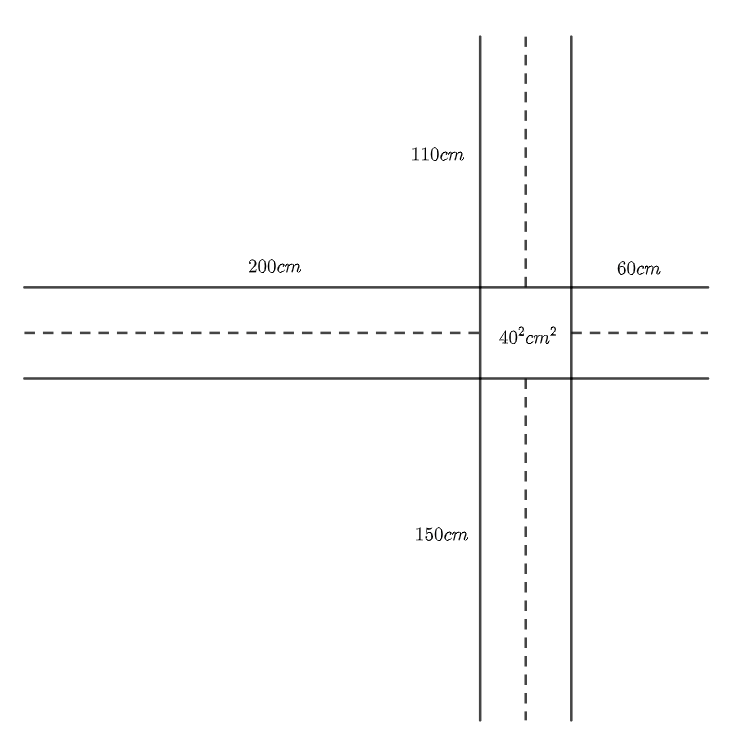
\includegraphics[width=1\linewidth]{figures/alt_intersection_config}
	\caption{An alternative configuration of the intersection and its connected roads by adding extra parameter to the initialization of the intersection as described by the previous code snippet.}
	\label{fig:altintersectionconfig}
\end{figure}

The length is in centimeters and needs to correlate with the length of the physical track. We used tape to show where the roads were. However, this is unnecessary. We recommend a track between three to four meters long for the best results.

Lastly, position both vehicles down at the start of the two tracks, turn on the server and connect to the power banks. The vehicles should automatically connect to the server after 20-30 seconds. When both vehicles have established a connection to the server, the demonstration has started.
% \section{Preface}

The product documentation is a technical description of the product.

The product documentation assumes the reader has some prior knowledge in basic programming.
% \section{Program description}

\begin{figure}[h!]
	\centering
	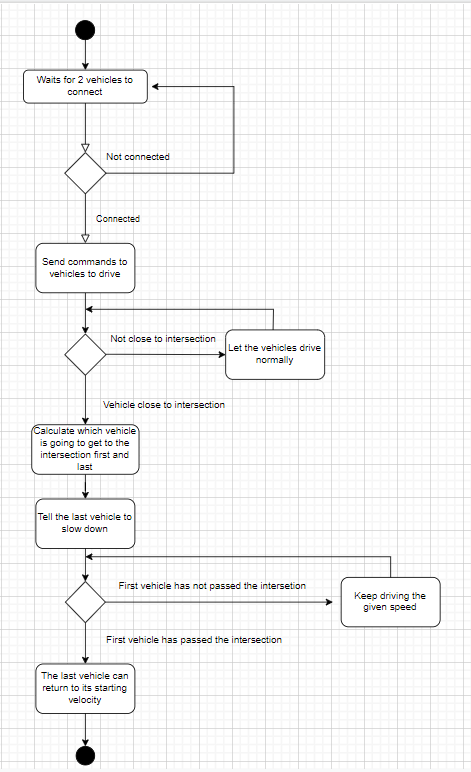
\includegraphics[width=1\linewidth]{figures/Flow_diagram_server}
	\caption[Flow diagram server]{Flow diagram for the server. This diagram specificly shows the flow of the semi physical demonstration.}
	\label{fig:diagramserver}
\end{figure}

The program is an IoT-system were vehicles can communicate with eachother through a server. It constists of a server which has the responsibility for the calculations and decision making, and a client which are the vehicles. The function of the program is to increase traffic flow and prevent traffic congestion. As of now the program can be used in an intersection with two vehicles, but can be scaled to include more vehicles. Here is a diagram that describes the flow of our server in the demonstration:




% \section{Adherence to project requirements}
Our solution adheres to the requirements Accenture set for us. Our prototype cars can work both with, and without being connected to a server. The server can handle multiple connections and adjust trafic based on the situation on the road. Through er deomnstration we also showed a situation where the outcome differs depending on if the cars are connected to the server or just driving on the on-board AI.


% \section{Server flow diagram}
\chapter{User manual}\label{sec:user_manual}
We have written a manual for people who want to recreate our demonstration. The demonstration could for example be shown off at exhibitions. The manual could also be used for people who want to further test and develop our IoT-system.

First check the IP-address of the internet you are connected to, and the usable ports. Make sure that your computer hosting the server and the vehicles are connected to the same network.

\begin{lstlisting}
$ipconfig getifaddr en0
192.168.56.208
\end{lstlisting}

Then open the Server solution in your code editor, we have used visual studio. Under the folder “properties” there is a file called launchSettings.json. In that file write in the ip address and the port in the applicationUrl-section:

\begin{json}
"profiles": {
	"SignalRServer": {
		"commandName": "Project",
		"dotnetRunMessages": true,
		"launchBrowser": false,
		"applicationUrl": "https://192.168.56.208:7058;http://192.168.56.208:5048",
		"environmentVariables": {
			"ASPNETCORE_ENVIRONMENT": "Development"
		}
	},
\end{json}
	
After that, open the Client solution. Here we used Pycharm as the IDE. Open the config.json document and replace the same IP address and port:
	
\begin{json}
"client": {
	"host": "192.168.56.208",
	"port": 5048,
	"delay": 0.1
},
\end{json}
	
	If the vehicles have not connected to that network before, they need to log on to that network. To log on to a new network; connect the Raspberry Pi to a power source and a display, and use the user interface. The display port on the Raspberry Pi is a micro USB port. When the Raspberry Pi has booted up, click on the internet icon and connect to the same network as the server. If the network has been connected to it before, Raspberry Pi will automatically connect to that network during boot up.
	
	The initial speed of the vehicles can be changed by adjusting the value of \verb|SpeedLimit| located at VehicleHubDatabase under the Database folder on the server solution:
\begin{csharp}
public class VehiclesHubDatabase : IVehiclesHubDatabase
{
	...
	public double SpeedLimit => 80;
	...
}
\end{csharp}
Moreover, the configuration of the road can also be changed by changing the following section of the code:
\begin{csharp}
public class VehiclesHubDatabase : IVehiclesHubDatabase
{
	...
	public VehiclesHubDatabase()
	{
		_intersection = new Intersection().
			AddRoad(new Road {Length = 300}.
				AddLane(null, true).
				AddLane()).
			AddRoad(new Road {Length = 300}.
				AddLane(null, true).
				AddLane());
		...
	}
	...
}
\end{csharp}
The current configuration shown above corresponds to the same configuration shown in \figref{fig:intersectionconcept}. The intersection can be moved by adding additional arguments such as:
\begin{csharp}
	public class VehiclesHubDatabase : IVehiclesHubDatabase
	{
		...
		public VehiclesHubDatabase()
		{
			_intersection = new Intersection().
				AddRoad(new Road {Length = 300}.
					AddLane(null, true).
					AddLane(), 200).
				AddRoad(new Road {Length = 300}.
					AddLane(null, true).
					AddLane(), 150);
			...
		}
		...
	}
\end{csharp}
\figref{fig:altintersectionconfig} shows the resulting topology by adding extra parameters to the code above.
\begin{figure}[h!]
	\centering
	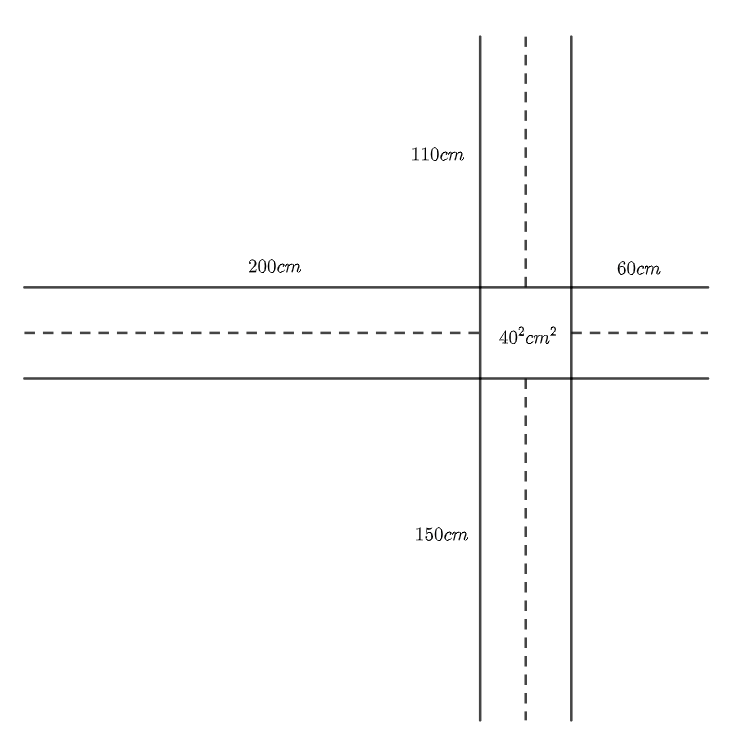
\includegraphics[width=1\linewidth]{figures/alt_intersection_config}
	\caption{An alternative configuration of the intersection and its connected roads by adding extra parameter to the initialization of the intersection as described by the previous code snippet.}
	\label{fig:altintersectionconfig}
\end{figure}

The length is in centimeters and needs to correlate with the length of the physical track. We used tape to show where the roads were. However, this is unnecessary. We recommend a track between three to four meters long for the best results.

Lastly, position both vehicles down at the start of the two tracks, turn on the server and connect to the power banks. The vehicles should automatically connect to the server after 20-30 seconds. When both vehicles have established a connection to the server, the demonstration has started.
\section{Product specification}
The main part of this project is to develop a client-server communication system, with the purpose of producing a physical simulation on how a centralized system can contribute to an improved traffic flow. Due to the nature of this project, no graphical user interfaces has been developed. Hence, it is deemed necessary to present key parts of the code that are responsible for such a system to work. This section will therefore elaborate, in detail, how essential code snippets are interacting with each to produce the result.

Furthermore, the code that has been written during this project has been written in the languages Python and C\# using Pycharm and Rider IDE respectively. Therefore, syntax highlighting has also been used to best simulate the same syntax highlighting used in both IDE respectively. In addition, some artistic freedom has been used to present the code snippets; the symbol \verb|...| has been used to indicate irrelevant code to the current discussion and the symbol  \textcolor{red}{$\hookrightarrow$} simply means that the line of code following \textcolor{red}{$\hookrightarrow$} is on the same line above but is broken up due to lack of space. Also, each code snippets starts with the class and method it belongs to.
\subsection{Initialization}\label{initialization}
\subsubsection{Client.py}
The client package is an essential module in the Raspberry Pi vehicles for the success of this project. The client class is mainly responsible for connecting, handling, and sending data to the server. The client class does not aim to be used alone but rather as a superclass for other IoT devices. Hence, it should be inherited and handle everything that pertains to client-server communication in the background.

The client's init method does several things: It reads from the config.json file to store the defined host and port it will use to establish a connection to the server.
\begin{python}
class Client:
	def __init__(self, properties=None, **kwargs):
		...
		with open("client/config.json") as f:
			config = json.load(f).get('client')
			if config is not None:
				self.__uri = f"://{config.get('host')}:{config.get('port')}/{self.__class__.__name__.lower()}sHub"
				self.__delay = config.get('delay')
		...
\end{python}

Then, it starts a negotiation process with the server, where it receives a connection id that the client will use during its connection lifetime to the hub.

\begin{python}
class Client:
	def __init__(self, properties=None, **kwargs):
		...
		urllib3.disable_warnings()
		response = requests.post(f"http{self.__uri}/negotiate?negotiateVersion=0", verify=False)
		self.connection_id = response.json().get("connectionId")
		self.websocket_uri = f"ws{self.__uri}?id={self.connection_id}"
		...
\end{python}

The client also gives itself a random id stored as one of its properties. The client's id is also stored on the server and is mainly used to retrieve and update the client's information.

Furthermore, \verb|Client.__init__| also stores a dictionary of events.
\begin{python}
class Client:
	def __init__(self, properties=None, **kwargs):
		...
		self.subscribed_events = {
			"disconnect": self.disconnect,
			"force_patch": self.force_patch,
			"continuously_patch": self.continuously_force_patch
		}
		...
\end{python}

Values in this dictionary are references to functions in this class and is used to invoke certain behaviours by the server. For instance, \newline\verb|await Clients.Client(Context.ConnectionId).SendAsync("disconnect");| from the server will call \verb|def disconnect(self)| in the client. 

\subsubsection{Vehicle.py}
The vehicle class contains all the data and methods of the vehicle. Furthermore, \verb|class Vehicle(Client)| inherits the client class which enables \verb|Vehicle| to perform all the necessary operations to establish connection upon initiation. An important remark is that \verb|Client| performs the negotiation to the server using endpoint \newline \verb|{self.__class__.__name__.lower()}sHub/negotiate?negotiateVersion=0| meaning that through inheritence and initialization of \verb|Vehicle|, the subclass negotiates with the endpoint  \verb|vehiclesHub/negotiate?negotiateVersion=0|, which is mapped in \verb|Program.cs| with
\begin{csharp}
...
app.MapHub<VehiclesHub>("/vehiclesHub");
...
\end{csharp}

Furthermore, \verb|Vehicle| also reads from \verb|config.json| to define it's initial properties with the snippet shown below:
\begin{python}
class Vehicle(Client):
	def __init__(self, properties=None, **kwargs):
		...
		if properties is None and len(kwargs) == 0:
			with open("client/config.json") as f:
				config = json.load(f).get('vehicle')
				if config is not None:
					self.properties.update(config)
		...
\end{python}

\verb|Vehicle| also utilizes the property builder of \verb|Client|.

\begin{python}
class Vehicle(Client):
	def __init__(self, properties=None, **kwargs):
		...
		self.property_builder(
			required={'length', 'height', 'width', 'mass'},
			optional={'velocity': 0, 'position': 0, 'travel_plan': None},
		)
		...
\end{python}

In short, the property builder is used to define the required properties of the vehicle class. The meaning is to restrict somewhat what data the vehicle class should contain. If one should directly initialize Vehicle without using config.json, one must assign values to length, height, width, and mass.

Lastly, \verb|Vehicle| adds subscribed events that the server can invoke:
\begin{python}
class Vehicle(Client):
	def __init__(self, properties=None, **kwargs):
		...
		self.subscribed_events.update({
			"adjust_velocity": self.adjust_velocity
		})
\end{python}

Likewise, as in \verb|Client|, should other events be required for a vehicle, one can add it to the dictionary as proposed above.
\subsection{Handshake and listener}\label{handshake}
After initializing the vehicle class as a client with
\begin{python}
async def main():
	...
	client = Vehicle()
	...
\end{python}
then the client's \verb|listen| method can be called:
\begin{python}
async def main():
	...
	listener = asyncio.create_task(client.listen())
	...
\end{python}
The listener method is responsible for handling responses and requests from the server. Hence, it must run concurrently as the vehicle continuously sends data to the server.

When the listener is called, the client performs the following code:
\begin{python}
class Client:
...
	async def listen(self):
	async with websockets.connect(self.websocket_uri) as websocket:
		self.__websocket = websocket
		await self.__handshake()
		await self.__listen()
...
\end{python}
The method first opens a WebSocket connection using the stored URI and stores this as a private variable. Then, a handshake with the server is performed:
\begin{python}
class Client:
...
	async def __handshake(self, protocol: str = "json", version: int = 1):
		data = self.signalr_encode_message({"protocol": protocol, "version": version})
		await self.__websocket.send(data)
		response = self.signalr_decode_message(await self.__websocket.recv())
		if "error" in response:
			print(response)
		else:
			await self.send_non_blocking("AddClient", self.properties)
...
\end{python}

The code above describes the handshake process between the client and the server. First, the client informs the server of the protocols it will use throughout its lifetime. Then, it stores the client, in this case, the vehicle, to the server using the defined properties.

Further elaboration, the client invokes the method
\begin{csharp}
public partial class VehiclesHub : Hub
{
	...
	public async Task AddClient(JsonDocument jsonDocument) {...}
	...
}
\end{csharp}
on the server. This method first creates a vehicle with all the provided information sent by the client
\begin{csharp}
public partial class VehiclesHub : Hub
{
	...
	public async Task AddClient(JsonDocument jsonDocument)
	{
		...
		var vehicle = Vehicle.Create(jsonDocument);
		...
	}
	...
}
\end{csharp}
using the static method defined by the Vehicle model. In addition, it assigns the travel plan to the vehicle by using values defined by config.json from the client:
\begin{json}
{
	...
	"vehicle": {
		...
		"travel_plan": {
			"start": {
				"road": 0,
				"lane_reversed": false
			},
			"end": {
				"road": 0,
				"lane_reversed": false
			}
		}
	}
}
\end{json}

Furthermore, the vehicle's current lane is also assigned to track which lane the vehicle is driving on. Then, \verb|public class VehiclesHubDatabase| adds the \verb|Vehicle|, together with its connection id \verb|Context.ConnectionId| for easy retrieval.

Moreover, for the sake of the demo, the server is also instructed to wait for a second vehicle to connect before allowing the vehicles to drive
\begin{csharp}
public partial class VehiclesHub : Hub
{
	...
	public async Task AddClient(JsonDocument jsonDocument)
	{
		...
		vehicle.Velocity = 0;
		_database.Update(vehicle);
		await Clients.Client(Context.ConnectionId).SendAsync("adjust_velocity", vehicle);
		await WaitForVehicles(vehicle, _database.SpeedLimit, 2);
	}
	...
}
\end{csharp}
by first setting the vehicle's velocity to zero, updating the new velocity in the database, and adjusting the velocity of the client to zero. Lastly, it calls the \verb|WaitForVehicles| method, which will adjust every client's velocity to the defined \verb|SpeedLimit| in \verb|VehiclesHubDatabase|.

\subsection{Patch}
After initialization and handshake elaborated in \hyperref[initialization]{\ref{initialization} Initialization} and \hyperref[handshake]{\ref{handshake} Handshake and listener} respectively, the Raspberry Pi vehicles starts to drive into an intersection simultaneously. Throughout the journey the cars are continuously patching to the server, by calling the client's \verb|async def send\_patch| method.

\begin{python}
class Client:
	...
	async def send_patch(self, **kwargs) -> None:
		if self.properties_has_changed(**kwargs) or self.__continuously_patch:
			await self.send_invocation("patch", self.properties)
		else:
			await asyncio.sleep(self.__delay)
\end{python}

As seen above \pythoninline{send\_patch} calls the \pythoninline{async def send_invocation} method, which communicates the vehicle's current information by invoking \newline
\verb|public async Task Patch| on \verb|VehiclesHub|.

The patch method on \verb|VehiclesHub| is responsible for handling the behaviour, specifically adjusting the velocity of individual vehicles:
\begin{csharp}
public partial class VehiclesHub : Hub
{
	...
	public async Task Patch(JsonDocument jsonDocument)
	{
		var vehicle = Vehicle.Create(jsonDocument);
		_database.Update(vehicle);
		vehicle = _database.Fetch(vehicle);
		...
	}
}
\end{csharp}
The snippet above shows that the method first creates a new vehicle using the information provided by the \verb|Client|. However, since this new vehicle does not contain all the information, such as the travel plan, the method first update the existing vehicle in the database in order to refresh the vehicle with the available information. It then fetch the same vehicle that was stored in the handshake, mentioned in \hyperref[handshake]{\ref{handshake} Handshake and listener}. Assuming that the vehicle has been successfully retrieved it will then handle this vehicle accordingly:
\begin{csharp}
public partial class VehiclesHub : Hub
{
	...
	public async Task Patch(JsonDocument jsonDocument)
	{
		...
		await HandleIntersection(vehicle);
		await HandleInsideIntersection(vehicle);
		await HandleEndOfRoute(vehicle);
		...
	}
}
\end{csharp}
Shortly summarized \verb|HandleIntersection| is responsible to adjust the velocity of every vehicle approaching the intersection to avoid collisions. Furthermore, \verb|HandleInsideIntersection| increases the speed to \verb|VehiclesHubDatabase| defined \verb|SpeedLimit|. Lastly, \verb|HandleEndOfRoute| ensure that any vehicles that has completed their journey, defined during the handshake, terminates their connection with the server.
\subsection{VehiclesHubDatabase}
The \verb|VehiclesHubDatabase| played a key role in this project. Coming to the realization on \hyperref[phase3]{\ref{phase3} Phase 3 - Signal R} the project needed a database that could handle the continuous changes in each \verb|Vehicle| position in real time. During research the group was unable to conclude on any databases that would fit our requirement. Hence, \verb|VehiclesHubDatanbase| was created to serve as a live in-memory database that could continuously update the positions of each vehicle on each lane.
\begin{figure}[h!]
	\centering
	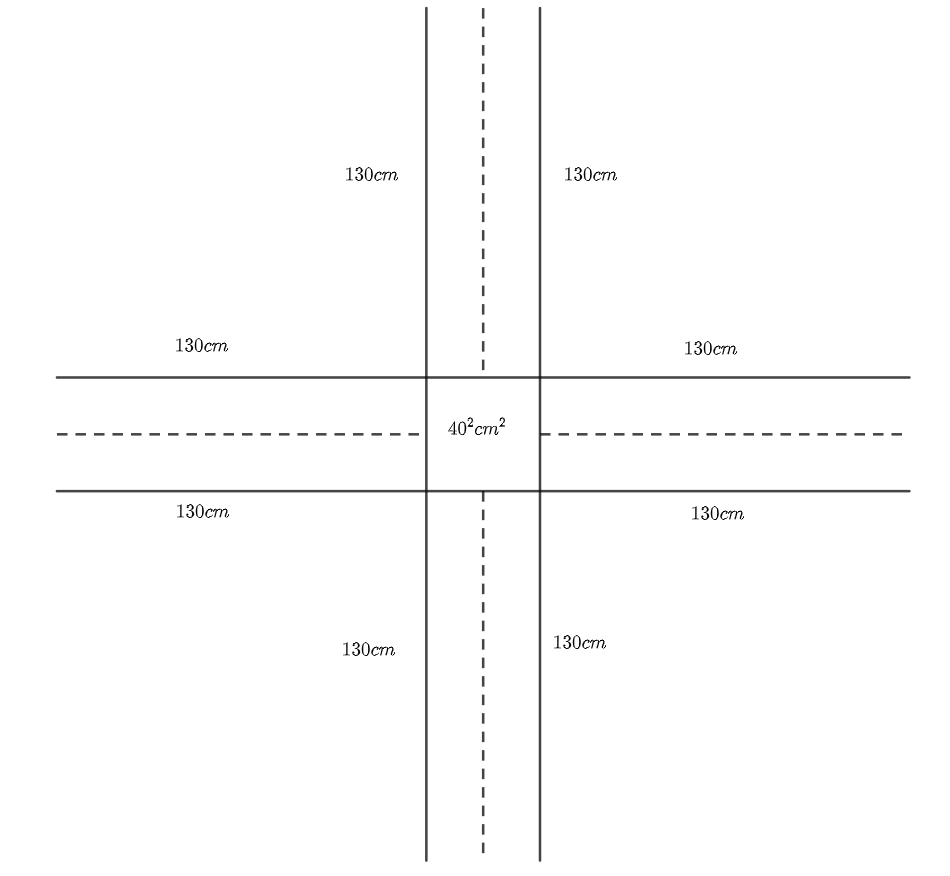
\includegraphics[width=1\linewidth]{figures/intersection_concept}
	\caption{This figure shows two roads each with two lanes and a total length of 300cm. The overlapping part forms a square which is the intersection. This configuration was heavily considered when creating representational models on the server, and also used for the demo as a result.}
	\label{fig:intersectionconcept}
\end{figure}

Before starting with \verb|VehiclesHubDatabase|, it was required to define what a road, lane and intersection is, respectively. Thus, \verb|Road.cs|, \verb|Lane.cs| and \verb|Intersection.cs| was developed. Consequently, \verb|VehiclesHubDatabase| was created.
\begin{csharp}
public class VehiclesHubDatabase : IVehiclesHubDatabase
{
	private readonly Intersection _intersection;
	
	private readonly HashSet<Vehicle> _vehicles = new();
	private readonly HashSet<Lane> _lanes = new();
	public int Count => _vehicles.Count;
	private readonly Dictionary<string, Vehicle> _connectionIds = new();
	private readonly Dictionary<Vehicle, string> _vehiclesConnectionId = new();
	...
	public double SpeedLimit => 80;
	...
}
\end{csharp}

Currently, \verb|VehiclesHubDatabase| only holds one intersection, due to time constraint this was not extended for a configuration with multiple intersections. Moreover, both vehicles and lanes are stored inside a hashset for fast retrieval. In addition, \verb|Count| is used in \verb|WaitForVehicles|, elaborated in sub-section \hyperref[handshake]{\ref{handshake} Handshake and listener}, and \verb|_connectionId| and \verb|_vehiclesConnectionId| is used during \verb|Patch| to invoke \verb|adjust_velocity| on individual vehicles. While, \verb|SpeedLimit| defines the upper speed vehicles are limited to on the two roads shown in \hyperref[fig:intersectionconcept]{Figure \ref{fig:intersectionconcept}}.

The road configuration found in \hyperref[fig:intersectionconcept]{Figure \ref{fig:intersectionconcept}} is defined in the constructor using a builder pattern.
\begin{csharp}
public class VehiclesHubDatabase : IVehiclesHubDatabase
{
	...
	public VehiclesHubDatabase()
	{
		_intersection = new Intersection().
			AddRoad(new Road {Length = 300}.
				AddLane(null, true).
				AddLane()).
		AddRoad(new Road {Length = 300}.
				AddLane(null, true).
				AddLane());
		
		_intersection.ConnectedLanes().
			ForEach(lane => _lanes.Add(lane));
	}
	...
}
\end{csharp}

Lastly, \verb|VehiclesHubDatabase| is added as a singleton service in \verb|Program.cs| to ensure that we have a static database throughout the lifetime of the program:
\begin{csharp}
...
builder.Services.AddSingleton<IVehiclesHubDatabase>(new VehiclesHubDatabase());
...
\end{csharp}

It is also worth to mention some of the core  functionalities of \verb|VehiclesHubDatabase|:

\subsubsection{Adding vehicles}
Calling the \verb|Add| method makes it possible to add vehicles:
\begin{csharp}
public class VehiclesHubDatabase : IVehiclesHubDatabase
{
	...
	public void Add(Vehicle vehicle, string? connectionId = null) {...}
	
	public void Add(Vehicle vehicle, Lane? lane = null) {...}
	...
}
\end{csharp}

\subsubsection{Removing vehicles}
Removing vehicles can be achieved by calling the \verb|Remove| method:
\begin{csharp}
public class VehiclesHubDatabase : IVehiclesHubDatabase
{
	...
	public void Remove(Vehicle vehicle) {...}
	...
}
\end{csharp}

\subsubsection{Updating vehicles}
Updating either a specific information of a vehicle or all vehicles can be done by calling the \verb|Update| method:
\begin{csharp}
public class VehiclesHubDatabase : IVehiclesHubDatabase
{
	...
	public void Update(Vehicle? vehicle = null) {...}
	...
}
\end{csharp}

\subsubsection{Fetching vehicles}
One can fetch an existing vehicle from the database by passing a vehicle with the same GUID with:
\begin{csharp}
public class VehiclesHubDatabase : IVehiclesHubDatabase
{
	...
	public Vehicle? Fetch(Vehicle vehicle) {...}
	...
}
\end{csharp}

\subsubsection{Get the connection Id of a particular vehicle}
By passing a vehicle into
\begin{csharp}
public class VehiclesHubDatabase : IVehiclesHubDatabase
{
	...
	public string? ConnectionId(Vehicle vehicle) {...}
	...
}
\end{csharp}
one can retrieve the connection Id that the given vehicle is using.

\subsubsection{Find vehicles approaching the intersection}
Maybe the most important feature of \verb|VehiclesHubDatabase| is the two method shown below:
\begin{csharp}
public class VehiclesHubDatabase : IVehiclesHubDatabase
{
	...
	public IEnumerable<Vehicle> NextVehiclesIn() {...}
	public IEnumerable<Vehicle> OnlyFirstIntoNextVehiclesIn() {...}
}
\end{csharp}
The first method \verb|NextVehiclesIn| returns a list of vehicles currently approaching the intersection defined in the constructor, ordered with respect to the vehicle closest to the intersection. The latter method \verb|OnlyFirstIntoNextVehiclesIn| returns an ordered list of the closest vehicle per lane.



%	\chapter{Discussion}

In addition to implementing the program, we also had discussions regarding the viability of the program. Here we will discuss our own process and how such and IoT-system would apply to the real world. We will use our own data as well as some research to reflect over the usability of an IoT system where self driving cars can communicate with eachother.

\subsection{Self evaluation}
As mentioned earlier in \secref{sec:dev_method}, we took inspiration from two agile frameworks: Scrum and Kanban, but chose to lean more towards scrum in the end. The use of Scrum helped us reach our goals. However, we could have included our external supervisors more in the Scrum process in hindsight. We could have done this by including them in sprint retrospective meetings and discussing what our following sprint goals should have been together.

The IoT system can handle more vehicles, but the road model does not fully support functionalities for having more intersections than we currently have in our demonstration. Because of the time constraint, we also found it challenging to focus on scalability. Hence, we instead focused on getting a working demonstration.  

One challenge was that our group could not meet as much as we had wished because of work. However, all the requirements in the MosCoW analysis (\figref{fig:moscowmethod}) were reached except for the features in the "can have" section. All in all, the group was satisfied with the process.

\subsection{Educational Value}
Developing said program has been a challenging process, which our group has learned a lot from. We all feel that we have evolved into better developers, and that we now would be better suited for solving such a project in the future. 

\section{Further work}
How to implement self-driving in society in the best way is a question that will take a long time to answer. Through our work with this proof-of-concept we believe we have made an addition to this discussion. Due to time constraints, we have chosen not to implement some features that would make the product work in a more complex environment. These features could be explored if this project were to be further developed. 

\subsection{Scalability}
When the knowledge and research has come further regarding AI, there may be a possibility for such an IoT system to be scaled for the real world. There is a need for less traffic in the cities and our results from this project shows that an IoT-system where cars can communicate through a server will increase traffic flow. Scalability is therefore important which we had in mind while coding the server and the client.

Our demo only contains two cars but our server is built in a way where multiple vehicles can connect to it. There are also possibilities to connect other devices to the server, for example traffic lights. However there are no specific functionalities regarding traffic lights on the server as of now. Scaling the IoT system for functionalities with traffic lights is a task for future development. Adding roads and making a more complex road system would also be a task for future development. 

\subsection{Extendability to the real world applications}
\subsubsection*{Edge computing}
In the future when self-driving vehicles become more prominent, and the 5G network becomes more available there could be a possibility for IoT-systems handling traffic management. Our group therefore did some research regarding how the system will extend to the real world’s applications. 

The IoT systems usually follow the fog or edge computing architecture with distributed or even decentralized concepts \parencite[pp 149]{iot_platforms}. This is to prevent overloading on servers handling a lot of data. 

One solution to distribution of data is that each road has one server responsible for their respective road. If a road is long it will be split into geographical areas where one server has responsibility for their geographical area. Intersections will have a server handling information from both road’s respective servers, since information from both servers are needed to make decisions in intersections.

In the traffic there are a lot of unforeseen situations that can happen. Traditional coding will not be able to cover every outcome in a traffic situation, therefore there will be a need for AI on the servers in addition to the cars. 
\subsection{Risk management}

%	\chapter{Conclusion}
\section{Results}
In regards to the problem statement in \secref{sec:problem_statement} and the goals for this project discussed in \secref{sec:goals}, we have been able to successfully create a centralized system that communicates that can communicate with autonomous vehicles. A significant change in velocity can lead to a disruption of traffic flow, as discussed in \secref{sec:traffic_congestion}. Through multiple semi-physical demonstrations discussed in \secref{sec:demo}, it was apparent that the server was able to contribute to an improved traffic flow by preemptively reducing vehicles' to the necessary speed to prevent collisions. Even though this project did only account for scenarios involving intersections, it is also from the exploration done throughout this project that autonomous vehicles, together with a centralized system, can be the answer for improving traffic flow in the future.

Furthermore, we received positive feedback after showing our supervisors and product-owner video snippets of the conducted demonstrations. Additionally, the product owner confirmed that our results adhered to the requirements set by Accenture.

\subsection{Real world scenario}

If we compare the data from the semi physical demonstration to a real world cenario were instead of 80 cm/h the cars would drive in 80 km/h prior to an intersection. In the real world, one of the cars would have to stop before a traffic light while the other could drive past the intersection. This would lead to a velocity change from 80 km/h to 0. In our scenario the car would only have to slow down to 55 km/h.

However there are more factors to consider in a real world scenario such as: curved roads, human mistakes and animals jumping onto the road.
\subsection{Possible improvements}
All the features in the MoSCoW method from \secref{sec:moscow_method}, "could have" to "won't have this time" are features for a future project, either for Accenture to improve or for a future bachelor project. Although it fulfilled the product requirements given by Accenture, there is room for improvement. For example, with the accuracy of the demo, specifically by doing more calibration tests and making a more accurate formula than we were able to produce (see \hyperref[eq:vprelationship]{equation \eqref{eq:vprelationship}}). Furthermore, changing the wheels and installing an edge TPU to exploit the existing AI model will result in a more predictable trajectory of the vehicles.

Our demo only contains two cars, but our server supports scenarios with multiple cars. There are also possibilities to connect other devices to the server, for example, traffic lights. However, there are no specific functionalities for other IoT devices on the server. Scaling the IoT system for functionalities with other IoT devices is a task for future development. Adding roads and making a more complex road system would also be a task for future development.

As mentioned, we made a semi-physical simulation. However, a virtual simulation would potentially yield more data for research while also exploring other more complex road configurations.

Due to this project's time constraints, we, for instance, did not integrate machine learning with our server. Integrating machine learning on the server could expand its different capabilities and make the project more scalable and applicable to a broader range of scenarios. Such integration is deemed valuable for the further extension of this project.

Making a viable product in the real world is a long way ahead and will require a lot more testing and implementation on a bigger scale. With the rise in availability of self-driving vehicles and the 5G network, there could be a possibility of IoT systems managing traffic. We explored the posibility of implementing multiple servers, each  having responsibility for their own geographical area, or an entire road. This follows the edge computing architecture, which is popular in IoT systems and describes distributed network devices that communicate to one centralized server through ``edge'' devices \parencite[pp 149]{iot_platforms}. We did not implement this in our program, but it was one of our main ideas for how we would scale the system to implement more roads.

Finally, we hope that our testing and research can be of value towards realizing autonomous cars and traffic management on such a scale.

\section{Further discussions}
In addition to implementing the program, we also had discussions regarding the viability of the program. Here we will discuss our process and how such an IoT system would apply to the real world. We will use our data and some research to reflect the usability of an IoT system where self-driving cars can communicate with each other.

\subsection{Self evaluation}
As mentioned earlier in \secref{sec:dev_method}, we took inspiration from two agile frameworks: Scrum and Kanban, but chose to lean more towards scrum in the end. The use of Scrum helped us reach our goals. However, we could have included our external supervisors more in the Scrum process in hindsight. We could have done this by including them in sprint retrospective meetings and discussing what our following sprint goals should have been together.

The IoT system can handle more vehicles, but the road model does not fully support functionalities for having more intersections than we currently have in our demonstration. Because of the time constraint, we also found it challenging to focus on scalability. Hence, we instead focused on getting a working demonstration.  

One challenge was that our group could not meet as much as we had wished because of work. However, all the requirements in the MosCoW analysis (\figref{fig:moscowmethod}) were reached except for the features in the "can have" section. All in all, the group was satisfied with the process.

\subsection{Educational Value}
Developing said program has been a challenging process, which our group has learned a lot from. We all feel that we have evolved into better developers, and that we now would be better suited for solving such a project in the future. 

\section{Further work}
How to implement self-driving in society in the best way is a question that will take a long time to answer. Through our work with this proof-of-concept we believe we have made an addition to this discussion. Due to time constraints, we have chosen not to implement some features that would make the product work in a more complex environment. These features could be explored if this project were to be further developed. 

\subsection{Scalability}
When the knowledge and research has come further regarding AI, there may be a possibility for such an IoT system to be scaled for the real world. There is a need for less traffic in the cities and our results from this project shows that an IoT-system where cars can communicate through a server will increase traffic flow. Scalability is therefore important which we had in mind while coding the server and the client.

Our demo only contains two cars but our server is built in a way where multiple vehicles can connect to it. There are also possibilities to connect other devices to the server, for example traffic lights. However there are no specific functionalities regarding traffic lights on the server as of now. Scaling the IoT system for functionalities with traffic lights is a task for future development. Adding roads and making a more complex road system would also be a task for future development. 

\subsection{Extendability to the real world applications}
\subsubsection*{Edge computing}
In the future when self-driving vehicles become more prominent, and the 5G network becomes more available there could be a possibility for IoT-systems handling traffic management. Our group therefore did some research regarding how the system will extend to the real world’s applications. 

The IoT systems usually follow the fog or edge computing architecture with distributed or even decentralized concepts \parencite[pp 149]{iot_platforms}. This is to prevent overloading on servers handling a lot of data. 

One solution to distribution of data is that each road has one server responsible for their respective road. If a road is long it will be split into geographical areas where one server has responsibility for their geographical area. Intersections will have a server handling information from both road’s respective servers, since information from both servers are needed to make decisions in intersections.

In the traffic there are a lot of unforeseen situations that can happen. Traditional coding will not be able to cover every outcome in a traffic situation, therefore there will be a need for AI on the servers in addition to the cars. 
\subsection{Risk management}
	
	% ------------------------------------------------------------
	\clearpage
    \addcontentsline{toc}{chapter}{Bibliography}
    \printbibliography
\end{document}
